\documentclass[a4paper]{book}
\usepackage{makeidx}
\usepackage{natbib}
\usepackage{graphicx}
\usepackage{multicol}
\usepackage{float}
\usepackage{listings}
\usepackage{color}
\usepackage{ifthen}
\usepackage[table]{xcolor}
\usepackage{textcomp}
\usepackage{alltt}
\usepackage{ifpdf}
\ifpdf
\usepackage[pdftex,
            pagebackref=true,
            colorlinks=true,
            linkcolor=blue,
            unicode
           ]{hyperref}
\else
\usepackage[ps2pdf,
            pagebackref=true,
            colorlinks=true,
            linkcolor=blue,
            unicode
           ]{hyperref}
\usepackage{pspicture}
\fi
\usepackage[utf8]{inputenc}
\usepackage{mathptmx}
\usepackage[scaled=.90]{helvet}
\usepackage{courier}
\usepackage{sectsty}
\usepackage[titles]{tocloft}
\usepackage{doxygen}
\lstset{language=C++,inputencoding=utf8,basicstyle=\footnotesize,breaklines=true,breakatwhitespace=true,tabsize=6,numbers=left }
\makeindex
\setcounter{tocdepth}{3}
\renewcommand{\footrulewidth}{0.4pt}
\renewcommand{\familydefault}{\sfdefault}
\hfuzz=15pt
\setlength{\emergencystretch}{15pt}
\hbadness=750
\tolerance=750
\begin{document}
\hypersetup{pageanchor=false,citecolor=blue}
\begin{titlepage}
\vspace*{7cm}
\begin{center}
{\Large \-S\-Q\-Lite\-Test \\[1ex]\large 0.\-3.\-0a }\\
\vspace*{1cm}
{\large \-Generated by Doxygen 1.7.6.1}\\
\vspace*{0.5cm}
{\small Tue Nov 13 2012 11:35:03}\\
\end{center}
\end{titlepage}
\clearemptydoublepage
\pagenumbering{roman}
\tableofcontents
\clearemptydoublepage
\pagenumbering{arabic}
\hypersetup{pageanchor=true,citecolor=blue}
\chapter{\-Namespace \-Index}
\section{\-Namespace \-List}
\-Here is a list of all namespaces with brief descriptions\-:\begin{DoxyCompactList}
\item\contentsline{section}{\hyperlink{namespacesqlitetest}{sqlitetest} }{\pageref{namespacesqlitetest}}{}
\item\contentsline{section}{\hyperlink{namespaceUi}{\-Ui} }{\pageref{namespaceUi}}{}
\end{DoxyCompactList}

\chapter{\-Class \-Index}
\section{\-Class \-List}
\-Here are the classes, structs, unions and interfaces with brief descriptions\-:\begin{DoxyCompactList}
\item\contentsline{section}{\hyperlink{classAboutDialog}{\-About\-Dialog} }{\pageref{classAboutDialog}}{}
\item\contentsline{section}{\hyperlink{classHelpSetDialog}{\-Help\-Set\-Dialog} }{\pageref{classHelpSetDialog}}{}
\item\contentsline{section}{\hyperlink{classMainWindow}{\-Main\-Window} }{\pageref{classMainWindow}}{}
\item\contentsline{section}{\hyperlink{classResultDialog}{\-Result\-Dialog} }{\pageref{classResultDialog}}{}
\item\contentsline{section}{\hyperlink{classSQLite}{\-S\-Q\-Lite} }{\pageref{classSQLite}}{}
\item\contentsline{section}{\hyperlink{structSqlPreferences}{\-Sql\-Preferences} }{\pageref{structSqlPreferences}}{}
\end{DoxyCompactList}

\chapter{\-File \-Index}
\section{\-File \-List}
\-Here is a list of all files with brief descriptions\-:\begin{DoxyCompactList}
\item\contentsline{section}{\hyperlink{aboutdialog_8cpp}{aboutdialog.\-cpp} }{\pageref{aboutdialog_8cpp}}{}
\item\contentsline{section}{\hyperlink{aboutdialog_8h}{aboutdialog.\-h} }{\pageref{aboutdialog_8h}}{}
\item\contentsline{section}{\hyperlink{helpsetdialog_8cpp}{helpsetdialog.\-cpp} }{\pageref{helpsetdialog_8cpp}}{}
\item\contentsline{section}{\hyperlink{helpsetdialog_8h}{helpsetdialog.\-h} }{\pageref{helpsetdialog_8h}}{}
\item\contentsline{section}{\hyperlink{main_8cpp}{main.\-cpp} }{\pageref{main_8cpp}}{}
\item\contentsline{section}{\hyperlink{mainwindow_8cpp}{mainwindow.\-cpp} }{\pageref{mainwindow_8cpp}}{}
\item\contentsline{section}{\hyperlink{mainwindow_8h}{mainwindow.\-h} }{\pageref{mainwindow_8h}}{}
\item\contentsline{section}{\hyperlink{resultdialog_8cpp}{resultdialog.\-cpp} }{\pageref{resultdialog_8cpp}}{}
\item\contentsline{section}{\hyperlink{resultdialog_8h}{resultdialog.\-h} }{\pageref{resultdialog_8h}}{}
\item\contentsline{section}{\hyperlink{sqlite_8cpp}{sqlite.\-cpp} }{\pageref{sqlite_8cpp}}{}
\item\contentsline{section}{\hyperlink{sqlite_8h}{sqlite.\-h} }{\pageref{sqlite_8h}}{}
\end{DoxyCompactList}

\chapter{\-Namespace \-Documentation}
\hypertarget{namespacesqlitetest}{\section{sqlitetest \-Namespace \-Reference}
\label{namespacesqlitetest}\index{sqlitetest@{sqlitetest}}
}


\subsection{\-Detailed \-Description}
\-S\-Q\-Lite\-Test -\/ \-Analysis \-Tools \-Kit

$\ast$$\ast$ \-Copyright (c) 2012 \-Emmodded \-Project \-All rights reserved.

\-This code is derived from software contributed to \-Emmodded \-Project by \-Maurizio \-Spoto $<$\href{mailto:mspoto@emmodded.org}{\tt mspoto@emmodded.\-org}$>$

\-Redistribution and use in source and binary forms, with or without modification, are permitted provided that the following conditions are met\-: 1. \-Redistributions of source code must retain the above copyright notice, this list of conditions and the following disclaimer. 2. \-Redistributions in binary form must reproduce the above copyright notice, this list of conditions and the following disclaimer in the documentation and/or other materials provided with the distribution.

\-T\-H\-I\-S \-S\-O\-F\-T\-W\-A\-R\-E \-I\-S \-P\-R\-O\-V\-I\-D\-E\-D \-B\-Y \-E\-M\-M\-O\-D\-D\-E\-D \-P\-R\-O\-J\-E\-C\-T \-A\-N\-D \-C\-O\-N\-T\-R\-I\-B\-U\-T\-O\-R\-S ``\-A\-S \-I\-S'' \-A\-N\-D \-A\-N\-Y \-E\-X\-P\-R\-E\-S\-S \-O\-R \-I\-M\-P\-L\-I\-E\-D \-W\-A\-R\-R\-A\-N\-T\-I\-E\-S, \-I\-N\-C\-L\-U\-D\-I\-N\-G, \-B\-U\-T \-N\-O\-T \-L\-I\-M\-I\-T\-E\-D \-T\-O, \-T\-H\-E \-I\-M\-P\-L\-I\-E\-D \-W\-A\-R\-R\-A\-N\-T\-I\-E\-S \-O\-F \-M\-E\-R\-C\-H\-A\-N\-T\-A\-B\-I\-L\-I\-T\-Y \-A\-N\-D \-F\-I\-T\-N\-E\-S\-S \-F\-O\-R \-A \-P\-A\-R\-T\-I\-C\-U\-L\-A\-R \-P\-U\-R\-P\-O\-S\-E \-A\-R\-E \-D\-I\-S\-C\-L\-A\-I\-M\-E\-D. \-I\-N \-N\-O \-E\-V\-E\-N\-T \-S\-H\-A\-L\-L \-T\-H\-E \-F\-O\-U\-N\-D\-A\-T\-I\-O\-N \-O\-R \-C\-O\-N\-T\-R\-I\-B\-U\-T\-O\-R\-S \-B\-E \-L\-I\-A\-B\-L\-E \-F\-O\-R \-A\-N\-Y \-D\-I\-R\-E\-C\-T, \-I\-N\-D\-I\-R\-E\-C\-T, \-I\-N\-C\-I\-D\-E\-N\-T\-A\-L, \-S\-P\-E\-C\-I\-A\-L, \-E\-X\-E\-M\-P\-L\-A\-R\-Y, \-O\-R \-C\-O\-N\-S\-E\-Q\-U\-E\-N\-T\-I\-A\-L \-D\-A\-M\-A\-G\-E\-S (\-I\-N\-C\-L\-U\-D\-I\-N\-G, \-B\-U\-T \-N\-O\-T \-L\-I\-M\-I\-T\-E\-D \-T\-O, \-P\-R\-O\-C\-U\-R\-E\-M\-E\-N\-T \-O\-F \-S\-U\-B\-S\-T\-I\-T\-U\-T\-E \-G\-O\-O\-D\-S \-O\-R \-S\-E\-R\-V\-I\-C\-E\-S; \-L\-O\-S\-S \-O\-F \-U\-S\-E, \-D\-A\-T\-A, \-O\-R \-P\-R\-O\-F\-I\-T\-S; \-O\-R \-B\-U\-S\-I\-N\-E\-S\-S \-I\-N\-T\-E\-R\-R\-U\-P\-T\-I\-O\-N) \-H\-O\-W\-E\-V\-E\-R \-C\-A\-U\-S\-E\-D \-A\-N\-D \-O\-N \-A\-N\-Y \-T\-H\-E\-O\-R\-Y \-O\-F \-L\-I\-A\-B\-I\-L\-I\-T\-Y, \-W\-H\-E\-T\-H\-E\-R \-I\-N \-C\-O\-N\-T\-R\-A\-C\-T, \-S\-T\-R\-I\-C\-T \-L\-I\-A\-B\-I\-L\-I\-T\-Y, \-O\-R \-T\-O\-R\-T (\-I\-N\-C\-L\-U\-D\-I\-N\-G \-N\-E\-G\-L\-I\-G\-E\-N\-C\-E \-O\-R \-O\-T\-H\-E\-R\-W\-I\-S\-E) \-A\-R\-I\-S\-I\-N\-G \-I\-N \-A\-N\-Y \-W\-A\-Y \-O\-U\-T \-O\-F \-T\-H\-E \-U\-S\-E \-O\-F \-T\-H\-I\-S \-S\-O\-F\-T\-W\-A\-R\-E, \-E\-V\-E\-N \-I\-F \-A\-D\-V\-I\-S\-E\-D \-O\-F \-T\-H\-E \-P\-O\-S\-S\-I\-B\-I\-L\-I\-T\-Y \-O\-F \-S\-U\-C\-H \-D\-A\-M\-A\-G\-E.

\begin{DoxyVersion}{\-Version}
0.\-3.\-0a 
\end{DoxyVersion}
\begin{DoxyAuthor}{\-Author}
\-Maurizio \-Spoto \-::\-R\-T\-O\-Skit\-:\-: 
\end{DoxyAuthor}

\hypertarget{namespaceUi}{\section{\-Ui \-Namespace \-Reference}
\label{namespaceUi}\index{\-Ui@{\-Ui}}
}

\chapter{\-Class \-Documentation}
\hypertarget{classAboutDialog}{\section{\-About\-Dialog \-Class \-Reference}
\label{classAboutDialog}\index{\-About\-Dialog@{\-About\-Dialog}}
}


{\ttfamily \#include $<$aboutdialog.\-h$>$}

\subsection*{\-Public \-Member \-Functions}
\begin{DoxyCompactItemize}
\item 
\hyperlink{classAboutDialog_ad96fc2ce8de7568ace543b7c69c71c56}{\-About\-Dialog} (\-Q\-Widget $\ast$parent=0)
\item 
\hyperlink{classAboutDialog_a3d87f5a26a175bb2573965c98af6d4ca}{$\sim$\-About\-Dialog} ()
\end{DoxyCompactItemize}


\subsection{\-Detailed \-Description}


\-Definition at line 46 of file aboutdialog.\-h.



\subsection{\-Constructor \& \-Destructor \-Documentation}
\hypertarget{classAboutDialog_ad96fc2ce8de7568ace543b7c69c71c56}{\index{\-About\-Dialog@{\-About\-Dialog}!\-About\-Dialog@{\-About\-Dialog}}
\index{\-About\-Dialog@{\-About\-Dialog}!AboutDialog@{\-About\-Dialog}}
\subsubsection[{\-About\-Dialog}]{\setlength{\rightskip}{0pt plus 5cm}{\bf \-About\-Dialog\-::\-About\-Dialog} (
\begin{DoxyParamCaption}
\item[{\-Q\-Widget $\ast$}]{parent = {\ttfamily 0}}
\end{DoxyParamCaption}
)\hspace{0.3cm}{\ttfamily  \mbox{[}explicit\mbox{]}}}}\label{classAboutDialog_ad96fc2ce8de7568ace543b7c69c71c56}


\-Definition at line 40 of file aboutdialog.\-cpp.

\hypertarget{classAboutDialog_a3d87f5a26a175bb2573965c98af6d4ca}{\index{\-About\-Dialog@{\-About\-Dialog}!$\sim$\-About\-Dialog@{$\sim$\-About\-Dialog}}
\index{$\sim$\-About\-Dialog@{$\sim$\-About\-Dialog}!AboutDialog@{\-About\-Dialog}}
\subsubsection[{$\sim$\-About\-Dialog}]{\setlength{\rightskip}{0pt plus 5cm}{\bf \-About\-Dialog\-::$\sim$\-About\-Dialog} (
\begin{DoxyParamCaption}
{}
\end{DoxyParamCaption}
)}}\label{classAboutDialog_a3d87f5a26a175bb2573965c98af6d4ca}


\-Definition at line 47 of file aboutdialog.\-cpp.



\-The documentation for this class was generated from the following files\-:\begin{DoxyCompactItemize}
\item 
\hyperlink{aboutdialog_8h}{aboutdialog.\-h}\item 
\hyperlink{aboutdialog_8cpp}{aboutdialog.\-cpp}\end{DoxyCompactItemize}

\hypertarget{classHelpSetDialog}{\section{\-Help\-Set\-Dialog \-Class \-Reference}
\label{classHelpSetDialog}\index{\-Help\-Set\-Dialog@{\-Help\-Set\-Dialog}}
}


{\ttfamily \#include $<$helpsetdialog.\-h$>$}

\subsection*{\-Public \-Slots}
\begin{DoxyCompactItemize}
\item 
void \hyperlink{classHelpSetDialog_a392d911572314f20320bf43e1c97dacd}{\-Clicked\-Home} ()
\item 
void \hyperlink{classHelpSetDialog_a9837a1246bd3dfdc6e1adee2a49f2157}{\-Clicked\-Git} ()
\item 
void \hyperlink{classHelpSetDialog_aa3c79e2757893a38dd2e53271376ddb3}{\-Clicked\-Close} ()
\item 
void \hyperlink{classHelpSetDialog_a7183c0405fa07f127a0a9abc6929a8c7}{\-Clicked\-Back} ()
\item 
void \hyperlink{classHelpSetDialog_a2c435b9d4baaaf700d68e2f3433be28d}{\-Clicked\-Forward} ()
\item 
void \hyperlink{classHelpSetDialog_a9c38de387e813f10d1783e9327fe4c5a}{\-Clicked\-Refresh} ()
\item 
void \hyperlink{classHelpSetDialog_ae381f3412a99fec40b901265d0b393c5}{\-Clicked\-H0} ()
\item 
void \hyperlink{classHelpSetDialog_a6c83306c35879d7d46af2b0e1818b0c1}{\-Clicked\-H1} ()
\item 
void \hyperlink{classHelpSetDialog_a21e7bb69468d2d75db0f7c106bdd66fa}{\-Clicked\-H2} ()
\item 
void \hyperlink{classHelpSetDialog_a67325da32306a5330c51639cbb793311}{\-Clicked\-H3} ()
\item 
void \hyperlink{classHelpSetDialog_af2e0e69fc351dce5a0982a1fca5730cf}{\-Clicked\-H4} ()
\item 
void \hyperlink{classHelpSetDialog_a0ef6a793476a27e4a452985d3264bf69}{\-Clicked\-H5} ()
\item 
void \hyperlink{classHelpSetDialog_adadd548eb11c585c0daf8df7d00e09c1}{\-Clicked\-H6} ()
\item 
void \hyperlink{classHelpSetDialog_ab672ac4bea4fd9d86e47dfe4c0359cc8}{\-Clicked\-H7} ()
\item 
void \hyperlink{classHelpSetDialog_aeb83aba8c60d5b6793f2c4f607be1323}{\-Clicked\-H8} ()
\end{DoxyCompactItemize}
\subsection*{\-Public \-Member \-Functions}
\begin{DoxyCompactItemize}
\item 
\hyperlink{classHelpSetDialog_a42eedf3d1994361844e27c2d5455fc85}{\-Help\-Set\-Dialog} (bool first\-Call, \-Q\-Widget $\ast$parent=0)
\item 
\hyperlink{classHelpSetDialog_a59391ca64da7949e23bb6d9ed900e2eb}{$\sim$\-Help\-Set\-Dialog} ()
\item 
void \hyperlink{classHelpSetDialog_a2d56d35a2a180de735942cc56d297fd3}{close\-Event} (\-Q\-Close\-Event $\ast$event)
\end{DoxyCompactItemize}


\subsection{\-Detailed \-Description}


\-Definition at line 50 of file helpsetdialog.\-h.



\subsection{\-Constructor \& \-Destructor \-Documentation}
\hypertarget{classHelpSetDialog_a42eedf3d1994361844e27c2d5455fc85}{\index{\-Help\-Set\-Dialog@{\-Help\-Set\-Dialog}!\-Help\-Set\-Dialog@{\-Help\-Set\-Dialog}}
\index{\-Help\-Set\-Dialog@{\-Help\-Set\-Dialog}!HelpSetDialog@{\-Help\-Set\-Dialog}}
\subsubsection[{\-Help\-Set\-Dialog}]{\setlength{\rightskip}{0pt plus 5cm}{\bf \-Help\-Set\-Dialog\-::\-Help\-Set\-Dialog} (
\begin{DoxyParamCaption}
\item[{bool}]{first\-Call, }
\item[{\-Q\-Widget $\ast$}]{parent = {\ttfamily 0}}
\end{DoxyParamCaption}
)\hspace{0.3cm}{\ttfamily  \mbox{[}explicit\mbox{]}}}}\label{classHelpSetDialog_a42eedf3d1994361844e27c2d5455fc85}


\-Definition at line 40 of file helpsetdialog.\-cpp.



\-Here is the call graph for this function\-:\nopagebreak
\begin{figure}[H]
\begin{center}
\leavevmode
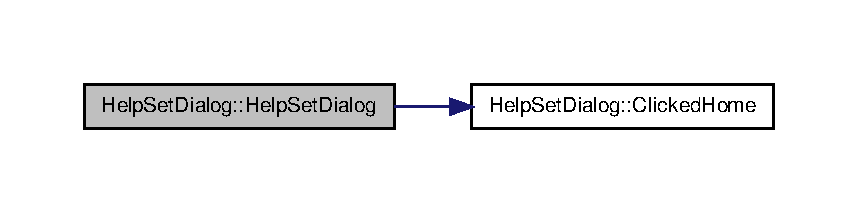
\includegraphics[width=350pt]{classHelpSetDialog_a42eedf3d1994361844e27c2d5455fc85_cgraph}
\end{center}
\end{figure}


\hypertarget{classHelpSetDialog_a59391ca64da7949e23bb6d9ed900e2eb}{\index{\-Help\-Set\-Dialog@{\-Help\-Set\-Dialog}!$\sim$\-Help\-Set\-Dialog@{$\sim$\-Help\-Set\-Dialog}}
\index{$\sim$\-Help\-Set\-Dialog@{$\sim$\-Help\-Set\-Dialog}!HelpSetDialog@{\-Help\-Set\-Dialog}}
\subsubsection[{$\sim$\-Help\-Set\-Dialog}]{\setlength{\rightskip}{0pt plus 5cm}{\bf \-Help\-Set\-Dialog\-::$\sim$\-Help\-Set\-Dialog} (
\begin{DoxyParamCaption}
{}
\end{DoxyParamCaption}
)}}\label{classHelpSetDialog_a59391ca64da7949e23bb6d9ed900e2eb}


\-Definition at line 52 of file helpsetdialog.\-cpp.



\subsection{\-Member \-Function \-Documentation}
\hypertarget{classHelpSetDialog_a7183c0405fa07f127a0a9abc6929a8c7}{\index{\-Help\-Set\-Dialog@{\-Help\-Set\-Dialog}!\-Clicked\-Back@{\-Clicked\-Back}}
\index{\-Clicked\-Back@{\-Clicked\-Back}!HelpSetDialog@{\-Help\-Set\-Dialog}}
\subsubsection[{\-Clicked\-Back}]{\setlength{\rightskip}{0pt plus 5cm}void {\bf \-Help\-Set\-Dialog\-::\-Clicked\-Back} (
\begin{DoxyParamCaption}
{}
\end{DoxyParamCaption}
)\hspace{0.3cm}{\ttfamily  \mbox{[}slot\mbox{]}}}}\label{classHelpSetDialog_a7183c0405fa07f127a0a9abc6929a8c7}


\-Definition at line 123 of file helpsetdialog.\-cpp.

\hypertarget{classHelpSetDialog_aa3c79e2757893a38dd2e53271376ddb3}{\index{\-Help\-Set\-Dialog@{\-Help\-Set\-Dialog}!\-Clicked\-Close@{\-Clicked\-Close}}
\index{\-Clicked\-Close@{\-Clicked\-Close}!HelpSetDialog@{\-Help\-Set\-Dialog}}
\subsubsection[{\-Clicked\-Close}]{\setlength{\rightskip}{0pt plus 5cm}void {\bf \-Help\-Set\-Dialog\-::\-Clicked\-Close} (
\begin{DoxyParamCaption}
{}
\end{DoxyParamCaption}
)\hspace{0.3cm}{\ttfamily  \mbox{[}slot\mbox{]}}}}\label{classHelpSetDialog_aa3c79e2757893a38dd2e53271376ddb3}


\-Definition at line 116 of file helpsetdialog.\-cpp.

\hypertarget{classHelpSetDialog_a2c435b9d4baaaf700d68e2f3433be28d}{\index{\-Help\-Set\-Dialog@{\-Help\-Set\-Dialog}!\-Clicked\-Forward@{\-Clicked\-Forward}}
\index{\-Clicked\-Forward@{\-Clicked\-Forward}!HelpSetDialog@{\-Help\-Set\-Dialog}}
\subsubsection[{\-Clicked\-Forward}]{\setlength{\rightskip}{0pt plus 5cm}void {\bf \-Help\-Set\-Dialog\-::\-Clicked\-Forward} (
\begin{DoxyParamCaption}
{}
\end{DoxyParamCaption}
)\hspace{0.3cm}{\ttfamily  \mbox{[}slot\mbox{]}}}}\label{classHelpSetDialog_a2c435b9d4baaaf700d68e2f3433be28d}


\-Definition at line 126 of file helpsetdialog.\-cpp.

\hypertarget{classHelpSetDialog_a9837a1246bd3dfdc6e1adee2a49f2157}{\index{\-Help\-Set\-Dialog@{\-Help\-Set\-Dialog}!\-Clicked\-Git@{\-Clicked\-Git}}
\index{\-Clicked\-Git@{\-Clicked\-Git}!HelpSetDialog@{\-Help\-Set\-Dialog}}
\subsubsection[{\-Clicked\-Git}]{\setlength{\rightskip}{0pt plus 5cm}void {\bf \-Help\-Set\-Dialog\-::\-Clicked\-Git} (
\begin{DoxyParamCaption}
{}
\end{DoxyParamCaption}
)\hspace{0.3cm}{\ttfamily  \mbox{[}slot\mbox{]}}}}\label{classHelpSetDialog_a9837a1246bd3dfdc6e1adee2a49f2157}


\-Definition at line 143 of file helpsetdialog.\-cpp.

\hypertarget{classHelpSetDialog_ae381f3412a99fec40b901265d0b393c5}{\index{\-Help\-Set\-Dialog@{\-Help\-Set\-Dialog}!\-Clicked\-H0@{\-Clicked\-H0}}
\index{\-Clicked\-H0@{\-Clicked\-H0}!HelpSetDialog@{\-Help\-Set\-Dialog}}
\subsubsection[{\-Clicked\-H0}]{\setlength{\rightskip}{0pt plus 5cm}void {\bf \-Help\-Set\-Dialog\-::\-Clicked\-H0} (
\begin{DoxyParamCaption}
{}
\end{DoxyParamCaption}
)\hspace{0.3cm}{\ttfamily  \mbox{[}slot\mbox{]}}}}\label{classHelpSetDialog_ae381f3412a99fec40b901265d0b393c5}


\-Definition at line 150 of file helpsetdialog.\-cpp.

\hypertarget{classHelpSetDialog_a6c83306c35879d7d46af2b0e1818b0c1}{\index{\-Help\-Set\-Dialog@{\-Help\-Set\-Dialog}!\-Clicked\-H1@{\-Clicked\-H1}}
\index{\-Clicked\-H1@{\-Clicked\-H1}!HelpSetDialog@{\-Help\-Set\-Dialog}}
\subsubsection[{\-Clicked\-H1}]{\setlength{\rightskip}{0pt plus 5cm}void {\bf \-Help\-Set\-Dialog\-::\-Clicked\-H1} (
\begin{DoxyParamCaption}
{}
\end{DoxyParamCaption}
)\hspace{0.3cm}{\ttfamily  \mbox{[}slot\mbox{]}}}}\label{classHelpSetDialog_a6c83306c35879d7d46af2b0e1818b0c1}


\-Definition at line 156 of file helpsetdialog.\-cpp.

\hypertarget{classHelpSetDialog_a21e7bb69468d2d75db0f7c106bdd66fa}{\index{\-Help\-Set\-Dialog@{\-Help\-Set\-Dialog}!\-Clicked\-H2@{\-Clicked\-H2}}
\index{\-Clicked\-H2@{\-Clicked\-H2}!HelpSetDialog@{\-Help\-Set\-Dialog}}
\subsubsection[{\-Clicked\-H2}]{\setlength{\rightskip}{0pt plus 5cm}void {\bf \-Help\-Set\-Dialog\-::\-Clicked\-H2} (
\begin{DoxyParamCaption}
{}
\end{DoxyParamCaption}
)\hspace{0.3cm}{\ttfamily  \mbox{[}slot\mbox{]}}}}\label{classHelpSetDialog_a21e7bb69468d2d75db0f7c106bdd66fa}


\-Definition at line 162 of file helpsetdialog.\-cpp.

\hypertarget{classHelpSetDialog_a67325da32306a5330c51639cbb793311}{\index{\-Help\-Set\-Dialog@{\-Help\-Set\-Dialog}!\-Clicked\-H3@{\-Clicked\-H3}}
\index{\-Clicked\-H3@{\-Clicked\-H3}!HelpSetDialog@{\-Help\-Set\-Dialog}}
\subsubsection[{\-Clicked\-H3}]{\setlength{\rightskip}{0pt plus 5cm}void {\bf \-Help\-Set\-Dialog\-::\-Clicked\-H3} (
\begin{DoxyParamCaption}
{}
\end{DoxyParamCaption}
)\hspace{0.3cm}{\ttfamily  \mbox{[}slot\mbox{]}}}}\label{classHelpSetDialog_a67325da32306a5330c51639cbb793311}


\-Definition at line 168 of file helpsetdialog.\-cpp.

\hypertarget{classHelpSetDialog_af2e0e69fc351dce5a0982a1fca5730cf}{\index{\-Help\-Set\-Dialog@{\-Help\-Set\-Dialog}!\-Clicked\-H4@{\-Clicked\-H4}}
\index{\-Clicked\-H4@{\-Clicked\-H4}!HelpSetDialog@{\-Help\-Set\-Dialog}}
\subsubsection[{\-Clicked\-H4}]{\setlength{\rightskip}{0pt plus 5cm}void {\bf \-Help\-Set\-Dialog\-::\-Clicked\-H4} (
\begin{DoxyParamCaption}
{}
\end{DoxyParamCaption}
)\hspace{0.3cm}{\ttfamily  \mbox{[}slot\mbox{]}}}}\label{classHelpSetDialog_af2e0e69fc351dce5a0982a1fca5730cf}


\-Definition at line 175 of file helpsetdialog.\-cpp.

\hypertarget{classHelpSetDialog_a0ef6a793476a27e4a452985d3264bf69}{\index{\-Help\-Set\-Dialog@{\-Help\-Set\-Dialog}!\-Clicked\-H5@{\-Clicked\-H5}}
\index{\-Clicked\-H5@{\-Clicked\-H5}!HelpSetDialog@{\-Help\-Set\-Dialog}}
\subsubsection[{\-Clicked\-H5}]{\setlength{\rightskip}{0pt plus 5cm}void {\bf \-Help\-Set\-Dialog\-::\-Clicked\-H5} (
\begin{DoxyParamCaption}
{}
\end{DoxyParamCaption}
)\hspace{0.3cm}{\ttfamily  \mbox{[}slot\mbox{]}}}}\label{classHelpSetDialog_a0ef6a793476a27e4a452985d3264bf69}


\-Definition at line 181 of file helpsetdialog.\-cpp.

\hypertarget{classHelpSetDialog_adadd548eb11c585c0daf8df7d00e09c1}{\index{\-Help\-Set\-Dialog@{\-Help\-Set\-Dialog}!\-Clicked\-H6@{\-Clicked\-H6}}
\index{\-Clicked\-H6@{\-Clicked\-H6}!HelpSetDialog@{\-Help\-Set\-Dialog}}
\subsubsection[{\-Clicked\-H6}]{\setlength{\rightskip}{0pt plus 5cm}void {\bf \-Help\-Set\-Dialog\-::\-Clicked\-H6} (
\begin{DoxyParamCaption}
{}
\end{DoxyParamCaption}
)\hspace{0.3cm}{\ttfamily  \mbox{[}slot\mbox{]}}}}\label{classHelpSetDialog_adadd548eb11c585c0daf8df7d00e09c1}


\-Definition at line 187 of file helpsetdialog.\-cpp.

\hypertarget{classHelpSetDialog_ab672ac4bea4fd9d86e47dfe4c0359cc8}{\index{\-Help\-Set\-Dialog@{\-Help\-Set\-Dialog}!\-Clicked\-H7@{\-Clicked\-H7}}
\index{\-Clicked\-H7@{\-Clicked\-H7}!HelpSetDialog@{\-Help\-Set\-Dialog}}
\subsubsection[{\-Clicked\-H7}]{\setlength{\rightskip}{0pt plus 5cm}void {\bf \-Help\-Set\-Dialog\-::\-Clicked\-H7} (
\begin{DoxyParamCaption}
{}
\end{DoxyParamCaption}
)\hspace{0.3cm}{\ttfamily  \mbox{[}slot\mbox{]}}}}\label{classHelpSetDialog_ab672ac4bea4fd9d86e47dfe4c0359cc8}


\-Definition at line 194 of file helpsetdialog.\-cpp.

\hypertarget{classHelpSetDialog_aeb83aba8c60d5b6793f2c4f607be1323}{\index{\-Help\-Set\-Dialog@{\-Help\-Set\-Dialog}!\-Clicked\-H8@{\-Clicked\-H8}}
\index{\-Clicked\-H8@{\-Clicked\-H8}!HelpSetDialog@{\-Help\-Set\-Dialog}}
\subsubsection[{\-Clicked\-H8}]{\setlength{\rightskip}{0pt plus 5cm}void {\bf \-Help\-Set\-Dialog\-::\-Clicked\-H8} (
\begin{DoxyParamCaption}
{}
\end{DoxyParamCaption}
)\hspace{0.3cm}{\ttfamily  \mbox{[}slot\mbox{]}}}}\label{classHelpSetDialog_aeb83aba8c60d5b6793f2c4f607be1323}


\-Definition at line 202 of file helpsetdialog.\-cpp.

\hypertarget{classHelpSetDialog_a392d911572314f20320bf43e1c97dacd}{\index{\-Help\-Set\-Dialog@{\-Help\-Set\-Dialog}!\-Clicked\-Home@{\-Clicked\-Home}}
\index{\-Clicked\-Home@{\-Clicked\-Home}!HelpSetDialog@{\-Help\-Set\-Dialog}}
\subsubsection[{\-Clicked\-Home}]{\setlength{\rightskip}{0pt plus 5cm}void {\bf \-Help\-Set\-Dialog\-::\-Clicked\-Home} (
\begin{DoxyParamCaption}
{}
\end{DoxyParamCaption}
)\hspace{0.3cm}{\ttfamily  \mbox{[}slot\mbox{]}}}}\label{classHelpSetDialog_a392d911572314f20320bf43e1c97dacd}


\-Definition at line 133 of file helpsetdialog.\-cpp.



\-Here is the caller graph for this function\-:\nopagebreak
\begin{figure}[H]
\begin{center}
\leavevmode
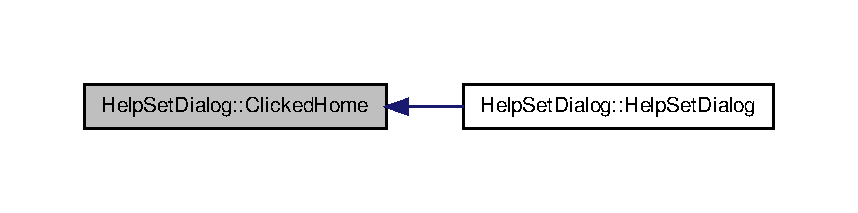
\includegraphics[width=350pt]{classHelpSetDialog_a392d911572314f20320bf43e1c97dacd_icgraph}
\end{center}
\end{figure}


\hypertarget{classHelpSetDialog_a9c38de387e813f10d1783e9327fe4c5a}{\index{\-Help\-Set\-Dialog@{\-Help\-Set\-Dialog}!\-Clicked\-Refresh@{\-Clicked\-Refresh}}
\index{\-Clicked\-Refresh@{\-Clicked\-Refresh}!HelpSetDialog@{\-Help\-Set\-Dialog}}
\subsubsection[{\-Clicked\-Refresh}]{\setlength{\rightskip}{0pt plus 5cm}void {\bf \-Help\-Set\-Dialog\-::\-Clicked\-Refresh} (
\begin{DoxyParamCaption}
{}
\end{DoxyParamCaption}
)\hspace{0.3cm}{\ttfamily  \mbox{[}slot\mbox{]}}}}\label{classHelpSetDialog_a9c38de387e813f10d1783e9327fe4c5a}


\-Definition at line 120 of file helpsetdialog.\-cpp.

\hypertarget{classHelpSetDialog_a2d56d35a2a180de735942cc56d297fd3}{\index{\-Help\-Set\-Dialog@{\-Help\-Set\-Dialog}!close\-Event@{close\-Event}}
\index{close\-Event@{close\-Event}!HelpSetDialog@{\-Help\-Set\-Dialog}}
\subsubsection[{close\-Event}]{\setlength{\rightskip}{0pt plus 5cm}void {\bf \-Help\-Set\-Dialog\-::close\-Event} (
\begin{DoxyParamCaption}
\item[{\-Q\-Close\-Event $\ast$}]{event}
\end{DoxyParamCaption}
)}}\label{classHelpSetDialog_a2d56d35a2a180de735942cc56d297fd3}


\-Definition at line 92 of file helpsetdialog.\-cpp.



\-The documentation for this class was generated from the following files\-:\begin{DoxyCompactItemize}
\item 
\hyperlink{helpsetdialog_8h}{helpsetdialog.\-h}\item 
\hyperlink{helpsetdialog_8cpp}{helpsetdialog.\-cpp}\end{DoxyCompactItemize}

\hypertarget{classMainWindow}{\section{\-Main\-Window \-Class \-Reference}
\label{classMainWindow}\index{\-Main\-Window@{\-Main\-Window}}
}


{\ttfamily \#include $<$mainwindow.\-h$>$}



\-Collaboration diagram for \-Main\-Window\-:\nopagebreak
\begin{figure}[H]
\begin{center}
\leavevmode
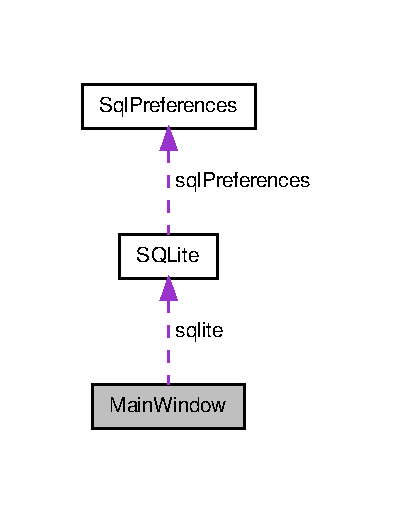
\includegraphics[width=190pt]{classMainWindow__coll__graph}
\end{center}
\end{figure}
\subsection*{\-Public \-Slots}
\begin{DoxyCompactItemize}
\item 
void \hyperlink{classMainWindow_aa58e3ed6d26ed5b593560bbf0f8f183c}{set\-Value\-E\-P\-S} (int value)
\item 
void \hyperlink{classMainWindow_a65c01e2454356623735a1ab596210304}{set\-Value\-S\-T} (int value)
\item 
void \hyperlink{classMainWindow_a75915c5f4286c3cdb3a7b0b3c240877a}{\-Change\-F\-F\-Gfield\-Type} (int)
\item 
void \hyperlink{classMainWindow_a22b08e83650062d966d3765b972fbc71}{\-Change\-F\-F\-Gfield\-Content} (int)
\item 
void \hyperlink{classMainWindow_a6e9f5e24aedd12d81b21148576a81b52}{\-Clicked\-Clear} ()
\item 
void \hyperlink{classMainWindow_a08902ba306b0d0aa85f02946edcb7a25}{\-Clicked\-Make} ()
\item 
void \hyperlink{classMainWindow_a2829d4a6fd7676b59809e9dd8f792fd6}{\-Clicked\-T\-E\-S\-T\-I\-N\-S\-E\-R\-T} ()
\item 
void \hyperlink{classMainWindow_a45d0243661d09bfc99392c94b0060060}{\-Clicked\-T\-E\-S\-T\-U\-P\-D\-A\-T\-E} ()
\item 
void \hyperlink{classMainWindow_a606b89316359652899d63d44b6cb86cf}{\-Clicked\-T\-E\-S\-T\-D\-E\-L\-E\-T\-E} ()
\item 
void \hyperlink{classMainWindow_a7908356fbc84a236502baf0f0bdbbe5c}{\-Clicked\-T\-E\-S\-T\-S\-E\-L\-E\-C\-T} ()
\item 
void \hyperlink{classMainWindow_a7be6a5d98970ac1a6296c6f9aee1e9bb}{about} ()
\item 
void \hyperlink{classMainWindow_aa7473e4bbbcc281706ac2edef864fb45}{open} ()
\item 
void \hyperlink{classMainWindow_a6532900ddf54d3587f12607a858cfff4}{run\-Timer\-Insert\-Event} ()
\item 
void \hyperlink{classMainWindow_ad751cceac9d285bd49518fccf7d7e018}{run\-Timer\-Update\-Event} ()
\item 
void \hyperlink{classMainWindow_a012e372e5d6180e36e3b08d27eaa6c36}{run\-Timer\-Delete\-Event} ()
\item 
void \hyperlink{classMainWindow_a124c316d7016496cbdc44a798cb26309}{run\-Timer\-Select\-Event} ()
\end{DoxyCompactItemize}
\subsection*{\-Public \-Member \-Functions}
\begin{DoxyCompactItemize}
\item 
\hyperlink{classMainWindow_a8b244be8b7b7db1b08de2a2acb9409db}{\-Main\-Window} (\-Q\-Widget $\ast$parent=0)
\item 
\hyperlink{classMainWindow_ae98d00a93bc118200eeef9f9bba1dba7}{$\sim$\-Main\-Window} ()
\end{DoxyCompactItemize}
\subsection*{\-Public \-Attributes}
\begin{DoxyCompactItemize}
\item 
\hyperlink{classSQLite}{\-S\-Q\-Lite} $\ast$ \hyperlink{classMainWindow_acd9e528f003b22f3c17657a89505803a}{sqlite}
\item 
int \hyperlink{classMainWindow_a271013fd9b8f471aed5ce6ff2941a6cf}{post\-Tmp\-Nrecords}
\item 
int \hyperlink{classMainWindow_a6c309625ea8d8bd81d552a96ffbbf368}{post\-Tmp\-Run\-Seconds}
\item 
bool \hyperlink{classMainWindow_ac3f3016f1a0ad93767c521c2fd349c7b}{full\-Speed}
\item 
int \hyperlink{classMainWindow_ac4e4dd0ba3dd8b958d2aec2271bfe299}{\-R\-R\-Lbytes}
\item 
int \hyperlink{classMainWindow_af648bf6238ec163343b5dec5e900fc23}{\-D\-R\-Lbytes}
\item 
bool \hyperlink{classMainWindow_a88b9fd4866e9ab0c99f50c7c0801e8de}{is\-Query\-Error}
\item 
\-Q\-String \hyperlink{classMainWindow_afbc3735a35d28cf9ce9a9873aacc4939}{query\-Error\-Msg}
\item 
\-Q\-List$<$ int $>$ \hyperlink{classMainWindow_a69d381f82b82ca37620172b78d58c4ea}{result\-Times}
\end{DoxyCompactItemize}


\subsection{\-Detailed \-Description}


\-Definition at line 64 of file mainwindow.\-h.



\subsection{\-Constructor \& \-Destructor \-Documentation}
\hypertarget{classMainWindow_a8b244be8b7b7db1b08de2a2acb9409db}{\index{\-Main\-Window@{\-Main\-Window}!\-Main\-Window@{\-Main\-Window}}
\index{\-Main\-Window@{\-Main\-Window}!MainWindow@{\-Main\-Window}}
\subsubsection[{\-Main\-Window}]{\setlength{\rightskip}{0pt plus 5cm}{\bf \-Main\-Window\-::\-Main\-Window} (
\begin{DoxyParamCaption}
\item[{\-Q\-Widget $\ast$}]{parent = {\ttfamily 0}}
\end{DoxyParamCaption}
)\hspace{0.3cm}{\ttfamily  \mbox{[}explicit\mbox{]}}}}\label{classMainWindow_a8b244be8b7b7db1b08de2a2acb9409db}


\-Definition at line 42 of file mainwindow.\-cpp.



\-Here is the call graph for this function\-:\nopagebreak
\begin{figure}[H]
\begin{center}
\leavevmode
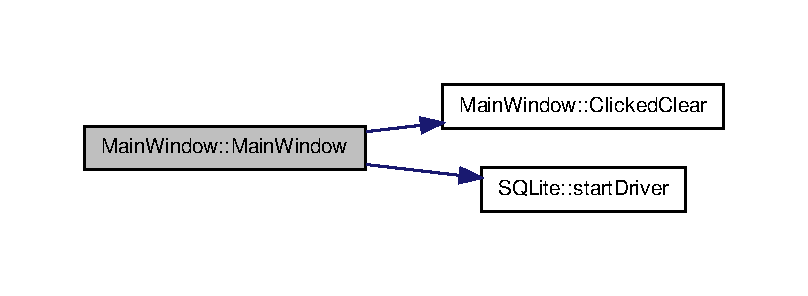
\includegraphics[width=350pt]{classMainWindow_a8b244be8b7b7db1b08de2a2acb9409db_cgraph}
\end{center}
\end{figure}


\hypertarget{classMainWindow_ae98d00a93bc118200eeef9f9bba1dba7}{\index{\-Main\-Window@{\-Main\-Window}!$\sim$\-Main\-Window@{$\sim$\-Main\-Window}}
\index{$\sim$\-Main\-Window@{$\sim$\-Main\-Window}!MainWindow@{\-Main\-Window}}
\subsubsection[{$\sim$\-Main\-Window}]{\setlength{\rightskip}{0pt plus 5cm}{\bf \-Main\-Window\-::$\sim$\-Main\-Window} (
\begin{DoxyParamCaption}
{}
\end{DoxyParamCaption}
)}}\label{classMainWindow_ae98d00a93bc118200eeef9f9bba1dba7}


\-Definition at line 57 of file mainwindow.\-cpp.



\-Here is the call graph for this function\-:\nopagebreak
\begin{figure}[H]
\begin{center}
\leavevmode
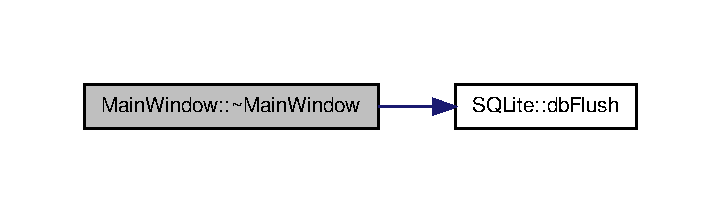
\includegraphics[width=346pt]{classMainWindow_ae98d00a93bc118200eeef9f9bba1dba7_cgraph}
\end{center}
\end{figure}




\subsection{\-Member \-Function \-Documentation}
\hypertarget{classMainWindow_a7be6a5d98970ac1a6296c6f9aee1e9bb}{\index{\-Main\-Window@{\-Main\-Window}!about@{about}}
\index{about@{about}!MainWindow@{\-Main\-Window}}
\subsubsection[{about}]{\setlength{\rightskip}{0pt plus 5cm}void {\bf \-Main\-Window\-::about} (
\begin{DoxyParamCaption}
{}
\end{DoxyParamCaption}
)\hspace{0.3cm}{\ttfamily  \mbox{[}slot\mbox{]}}}}\label{classMainWindow_a7be6a5d98970ac1a6296c6f9aee1e9bb}


\-Definition at line 836 of file mainwindow.\-cpp.

\hypertarget{classMainWindow_a22b08e83650062d966d3765b972fbc71}{\index{\-Main\-Window@{\-Main\-Window}!\-Change\-F\-F\-Gfield\-Content@{\-Change\-F\-F\-Gfield\-Content}}
\index{\-Change\-F\-F\-Gfield\-Content@{\-Change\-F\-F\-Gfield\-Content}!MainWindow@{\-Main\-Window}}
\subsubsection[{\-Change\-F\-F\-Gfield\-Content}]{\setlength{\rightskip}{0pt plus 5cm}void {\bf \-Main\-Window\-::\-Change\-F\-F\-Gfield\-Content} (
\begin{DoxyParamCaption}
\item[{int}]{}
\end{DoxyParamCaption}
)\hspace{0.3cm}{\ttfamily  \mbox{[}slot\mbox{]}}}}\label{classMainWindow_a22b08e83650062d966d3765b972fbc71}


\-Definition at line 809 of file mainwindow.\-cpp.

\hypertarget{classMainWindow_a75915c5f4286c3cdb3a7b0b3c240877a}{\index{\-Main\-Window@{\-Main\-Window}!\-Change\-F\-F\-Gfield\-Type@{\-Change\-F\-F\-Gfield\-Type}}
\index{\-Change\-F\-F\-Gfield\-Type@{\-Change\-F\-F\-Gfield\-Type}!MainWindow@{\-Main\-Window}}
\subsubsection[{\-Change\-F\-F\-Gfield\-Type}]{\setlength{\rightskip}{0pt plus 5cm}void {\bf \-Main\-Window\-::\-Change\-F\-F\-Gfield\-Type} (
\begin{DoxyParamCaption}
\item[{int}]{}
\end{DoxyParamCaption}
)\hspace{0.3cm}{\ttfamily  \mbox{[}slot\mbox{]}}}}\label{classMainWindow_a75915c5f4286c3cdb3a7b0b3c240877a}
\hypertarget{classMainWindow_MainWindow}{}\subsection{config}\label{classMainWindow_MainWindow}


\-Definition at line 793 of file mainwindow.\-cpp.

\hypertarget{classMainWindow_a6e9f5e24aedd12d81b21148576a81b52}{\index{\-Main\-Window@{\-Main\-Window}!\-Clicked\-Clear@{\-Clicked\-Clear}}
\index{\-Clicked\-Clear@{\-Clicked\-Clear}!MainWindow@{\-Main\-Window}}
\subsubsection[{\-Clicked\-Clear}]{\setlength{\rightskip}{0pt plus 5cm}void {\bf \-Main\-Window\-::\-Clicked\-Clear} (
\begin{DoxyParamCaption}
{}
\end{DoxyParamCaption}
)\hspace{0.3cm}{\ttfamily  \mbox{[}slot\mbox{]}}}}\label{classMainWindow_a6e9f5e24aedd12d81b21148576a81b52}


\-Definition at line 830 of file mainwindow.\-cpp.



\-Here is the caller graph for this function\-:\nopagebreak
\begin{figure}[H]
\begin{center}
\leavevmode
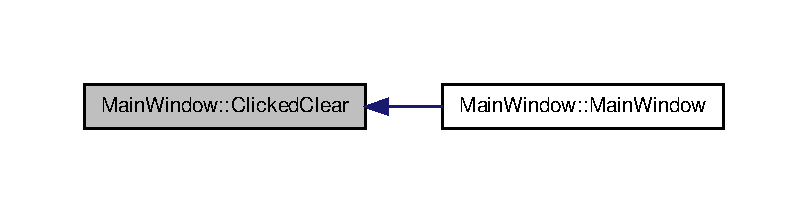
\includegraphics[width=350pt]{classMainWindow_a6e9f5e24aedd12d81b21148576a81b52_icgraph}
\end{center}
\end{figure}


\hypertarget{classMainWindow_a08902ba306b0d0aa85f02946edcb7a25}{\index{\-Main\-Window@{\-Main\-Window}!\-Clicked\-Make@{\-Clicked\-Make}}
\index{\-Clicked\-Make@{\-Clicked\-Make}!MainWindow@{\-Main\-Window}}
\subsubsection[{\-Clicked\-Make}]{\setlength{\rightskip}{0pt plus 5cm}void {\bf \-Main\-Window\-::\-Clicked\-Make} (
\begin{DoxyParamCaption}
{}
\end{DoxyParamCaption}
)\hspace{0.3cm}{\ttfamily  \mbox{[}slot\mbox{]}}}}\label{classMainWindow_a08902ba306b0d0aa85f02946edcb7a25}


\-Definition at line 833 of file mainwindow.\-cpp.

\hypertarget{classMainWindow_a606b89316359652899d63d44b6cb86cf}{\index{\-Main\-Window@{\-Main\-Window}!\-Clicked\-T\-E\-S\-T\-D\-E\-L\-E\-T\-E@{\-Clicked\-T\-E\-S\-T\-D\-E\-L\-E\-T\-E}}
\index{\-Clicked\-T\-E\-S\-T\-D\-E\-L\-E\-T\-E@{\-Clicked\-T\-E\-S\-T\-D\-E\-L\-E\-T\-E}!MainWindow@{\-Main\-Window}}
\subsubsection[{\-Clicked\-T\-E\-S\-T\-D\-E\-L\-E\-T\-E}]{\setlength{\rightskip}{0pt plus 5cm}void {\bf \-Main\-Window\-::\-Clicked\-T\-E\-S\-T\-D\-E\-L\-E\-T\-E} (
\begin{DoxyParamCaption}
{}
\end{DoxyParamCaption}
)\hspace{0.3cm}{\ttfamily  \mbox{[}slot\mbox{]}}}}\label{classMainWindow_a606b89316359652899d63d44b6cb86cf}


\-Definition at line 857 of file mainwindow.\-cpp.

\hypertarget{classMainWindow_a2829d4a6fd7676b59809e9dd8f792fd6}{\index{\-Main\-Window@{\-Main\-Window}!\-Clicked\-T\-E\-S\-T\-I\-N\-S\-E\-R\-T@{\-Clicked\-T\-E\-S\-T\-I\-N\-S\-E\-R\-T}}
\index{\-Clicked\-T\-E\-S\-T\-I\-N\-S\-E\-R\-T@{\-Clicked\-T\-E\-S\-T\-I\-N\-S\-E\-R\-T}!MainWindow@{\-Main\-Window}}
\subsubsection[{\-Clicked\-T\-E\-S\-T\-I\-N\-S\-E\-R\-T}]{\setlength{\rightskip}{0pt plus 5cm}void {\bf \-Main\-Window\-::\-Clicked\-T\-E\-S\-T\-I\-N\-S\-E\-R\-T} (
\begin{DoxyParamCaption}
{}
\end{DoxyParamCaption}
)\hspace{0.3cm}{\ttfamily  \mbox{[}slot\mbox{]}}}}\label{classMainWindow_a2829d4a6fd7676b59809e9dd8f792fd6}


\-Definition at line 851 of file mainwindow.\-cpp.

\hypertarget{classMainWindow_a7908356fbc84a236502baf0f0bdbbe5c}{\index{\-Main\-Window@{\-Main\-Window}!\-Clicked\-T\-E\-S\-T\-S\-E\-L\-E\-C\-T@{\-Clicked\-T\-E\-S\-T\-S\-E\-L\-E\-C\-T}}
\index{\-Clicked\-T\-E\-S\-T\-S\-E\-L\-E\-C\-T@{\-Clicked\-T\-E\-S\-T\-S\-E\-L\-E\-C\-T}!MainWindow@{\-Main\-Window}}
\subsubsection[{\-Clicked\-T\-E\-S\-T\-S\-E\-L\-E\-C\-T}]{\setlength{\rightskip}{0pt plus 5cm}void {\bf \-Main\-Window\-::\-Clicked\-T\-E\-S\-T\-S\-E\-L\-E\-C\-T} (
\begin{DoxyParamCaption}
{}
\end{DoxyParamCaption}
)\hspace{0.3cm}{\ttfamily  \mbox{[}slot\mbox{]}}}}\label{classMainWindow_a7908356fbc84a236502baf0f0bdbbe5c}


\-Definition at line 860 of file mainwindow.\-cpp.

\hypertarget{classMainWindow_a45d0243661d09bfc99392c94b0060060}{\index{\-Main\-Window@{\-Main\-Window}!\-Clicked\-T\-E\-S\-T\-U\-P\-D\-A\-T\-E@{\-Clicked\-T\-E\-S\-T\-U\-P\-D\-A\-T\-E}}
\index{\-Clicked\-T\-E\-S\-T\-U\-P\-D\-A\-T\-E@{\-Clicked\-T\-E\-S\-T\-U\-P\-D\-A\-T\-E}!MainWindow@{\-Main\-Window}}
\subsubsection[{\-Clicked\-T\-E\-S\-T\-U\-P\-D\-A\-T\-E}]{\setlength{\rightskip}{0pt plus 5cm}void {\bf \-Main\-Window\-::\-Clicked\-T\-E\-S\-T\-U\-P\-D\-A\-T\-E} (
\begin{DoxyParamCaption}
{}
\end{DoxyParamCaption}
)\hspace{0.3cm}{\ttfamily  \mbox{[}slot\mbox{]}}}}\label{classMainWindow_a45d0243661d09bfc99392c94b0060060}


\-Definition at line 854 of file mainwindow.\-cpp.

\hypertarget{classMainWindow_aa7473e4bbbcc281706ac2edef864fb45}{\index{\-Main\-Window@{\-Main\-Window}!open@{open}}
\index{open@{open}!MainWindow@{\-Main\-Window}}
\subsubsection[{open}]{\setlength{\rightskip}{0pt plus 5cm}void {\bf \-Main\-Window\-::open} (
\begin{DoxyParamCaption}
{}
\end{DoxyParamCaption}
)\hspace{0.3cm}{\ttfamily  \mbox{[}slot\mbox{]}}}}\label{classMainWindow_aa7473e4bbbcc281706ac2edef864fb45}


\-Definition at line 840 of file mainwindow.\-cpp.

\hypertarget{classMainWindow_a012e372e5d6180e36e3b08d27eaa6c36}{\index{\-Main\-Window@{\-Main\-Window}!run\-Timer\-Delete\-Event@{run\-Timer\-Delete\-Event}}
\index{run\-Timer\-Delete\-Event@{run\-Timer\-Delete\-Event}!MainWindow@{\-Main\-Window}}
\subsubsection[{run\-Timer\-Delete\-Event}]{\setlength{\rightskip}{0pt plus 5cm}void {\bf \-Main\-Window\-::run\-Timer\-Delete\-Event} (
\begin{DoxyParamCaption}
{}
\end{DoxyParamCaption}
)\hspace{0.3cm}{\ttfamily  \mbox{[}slot\mbox{]}}}}\label{classMainWindow_a012e372e5d6180e36e3b08d27eaa6c36}


\-Definition at line 754 of file mainwindow.\-cpp.

\hypertarget{classMainWindow_a6532900ddf54d3587f12607a858cfff4}{\index{\-Main\-Window@{\-Main\-Window}!run\-Timer\-Insert\-Event@{run\-Timer\-Insert\-Event}}
\index{run\-Timer\-Insert\-Event@{run\-Timer\-Insert\-Event}!MainWindow@{\-Main\-Window}}
\subsubsection[{run\-Timer\-Insert\-Event}]{\setlength{\rightskip}{0pt plus 5cm}void {\bf \-Main\-Window\-::run\-Timer\-Insert\-Event} (
\begin{DoxyParamCaption}
{}
\end{DoxyParamCaption}
)\hspace{0.3cm}{\ttfamily  \mbox{[}slot\mbox{]}}}}\label{classMainWindow_a6532900ddf54d3587f12607a858cfff4}


\-Definition at line 732 of file mainwindow.\-cpp.

\hypertarget{classMainWindow_a124c316d7016496cbdc44a798cb26309}{\index{\-Main\-Window@{\-Main\-Window}!run\-Timer\-Select\-Event@{run\-Timer\-Select\-Event}}
\index{run\-Timer\-Select\-Event@{run\-Timer\-Select\-Event}!MainWindow@{\-Main\-Window}}
\subsubsection[{run\-Timer\-Select\-Event}]{\setlength{\rightskip}{0pt plus 5cm}void {\bf \-Main\-Window\-::run\-Timer\-Select\-Event} (
\begin{DoxyParamCaption}
{}
\end{DoxyParamCaption}
)\hspace{0.3cm}{\ttfamily  \mbox{[}slot\mbox{]}}}}\label{classMainWindow_a124c316d7016496cbdc44a798cb26309}


\-Definition at line 743 of file mainwindow.\-cpp.

\hypertarget{classMainWindow_ad751cceac9d285bd49518fccf7d7e018}{\index{\-Main\-Window@{\-Main\-Window}!run\-Timer\-Update\-Event@{run\-Timer\-Update\-Event}}
\index{run\-Timer\-Update\-Event@{run\-Timer\-Update\-Event}!MainWindow@{\-Main\-Window}}
\subsubsection[{run\-Timer\-Update\-Event}]{\setlength{\rightskip}{0pt plus 5cm}void {\bf \-Main\-Window\-::run\-Timer\-Update\-Event} (
\begin{DoxyParamCaption}
{}
\end{DoxyParamCaption}
)\hspace{0.3cm}{\ttfamily  \mbox{[}slot\mbox{]}}}}\label{classMainWindow_ad751cceac9d285bd49518fccf7d7e018}


\-Definition at line 765 of file mainwindow.\-cpp.

\hypertarget{classMainWindow_aa58e3ed6d26ed5b593560bbf0f8f183c}{\index{\-Main\-Window@{\-Main\-Window}!set\-Value\-E\-P\-S@{set\-Value\-E\-P\-S}}
\index{set\-Value\-E\-P\-S@{set\-Value\-E\-P\-S}!MainWindow@{\-Main\-Window}}
\subsubsection[{set\-Value\-E\-P\-S}]{\setlength{\rightskip}{0pt plus 5cm}void {\bf \-Main\-Window\-::set\-Value\-E\-P\-S} (
\begin{DoxyParamCaption}
\item[{int}]{value}
\end{DoxyParamCaption}
)\hspace{0.3cm}{\ttfamily  \mbox{[}slot\mbox{]}}}}\label{classMainWindow_aa58e3ed6d26ed5b593560bbf0f8f183c}


\-Definition at line 824 of file mainwindow.\-cpp.

\hypertarget{classMainWindow_a65c01e2454356623735a1ab596210304}{\index{\-Main\-Window@{\-Main\-Window}!set\-Value\-S\-T@{set\-Value\-S\-T}}
\index{set\-Value\-S\-T@{set\-Value\-S\-T}!MainWindow@{\-Main\-Window}}
\subsubsection[{set\-Value\-S\-T}]{\setlength{\rightskip}{0pt plus 5cm}void {\bf \-Main\-Window\-::set\-Value\-S\-T} (
\begin{DoxyParamCaption}
\item[{int}]{value}
\end{DoxyParamCaption}
)\hspace{0.3cm}{\ttfamily  \mbox{[}slot\mbox{]}}}}\label{classMainWindow_a65c01e2454356623735a1ab596210304}


\-Definition at line 827 of file mainwindow.\-cpp.



\subsection{\-Member \-Data \-Documentation}
\hypertarget{classMainWindow_af648bf6238ec163343b5dec5e900fc23}{\index{\-Main\-Window@{\-Main\-Window}!\-D\-R\-Lbytes@{\-D\-R\-Lbytes}}
\index{\-D\-R\-Lbytes@{\-D\-R\-Lbytes}!MainWindow@{\-Main\-Window}}
\subsubsection[{\-D\-R\-Lbytes}]{\setlength{\rightskip}{0pt plus 5cm}int {\bf \-Main\-Window\-::\-D\-R\-Lbytes}}}\label{classMainWindow_af648bf6238ec163343b5dec5e900fc23}


\-Definition at line 76 of file mainwindow.\-h.

\hypertarget{classMainWindow_ac3f3016f1a0ad93767c521c2fd349c7b}{\index{\-Main\-Window@{\-Main\-Window}!full\-Speed@{full\-Speed}}
\index{full\-Speed@{full\-Speed}!MainWindow@{\-Main\-Window}}
\subsubsection[{full\-Speed}]{\setlength{\rightskip}{0pt plus 5cm}bool {\bf \-Main\-Window\-::full\-Speed}}}\label{classMainWindow_ac3f3016f1a0ad93767c521c2fd349c7b}


\-Definition at line 74 of file mainwindow.\-h.

\hypertarget{classMainWindow_a88b9fd4866e9ab0c99f50c7c0801e8de}{\index{\-Main\-Window@{\-Main\-Window}!is\-Query\-Error@{is\-Query\-Error}}
\index{is\-Query\-Error@{is\-Query\-Error}!MainWindow@{\-Main\-Window}}
\subsubsection[{is\-Query\-Error}]{\setlength{\rightskip}{0pt plus 5cm}bool {\bf \-Main\-Window\-::is\-Query\-Error}}}\label{classMainWindow_a88b9fd4866e9ab0c99f50c7c0801e8de}


\-Definition at line 77 of file mainwindow.\-h.

\hypertarget{classMainWindow_a271013fd9b8f471aed5ce6ff2941a6cf}{\index{\-Main\-Window@{\-Main\-Window}!post\-Tmp\-Nrecords@{post\-Tmp\-Nrecords}}
\index{post\-Tmp\-Nrecords@{post\-Tmp\-Nrecords}!MainWindow@{\-Main\-Window}}
\subsubsection[{post\-Tmp\-Nrecords}]{\setlength{\rightskip}{0pt plus 5cm}int {\bf \-Main\-Window\-::post\-Tmp\-Nrecords}}}\label{classMainWindow_a271013fd9b8f471aed5ce6ff2941a6cf}


\-Definition at line 72 of file mainwindow.\-h.

\hypertarget{classMainWindow_a6c309625ea8d8bd81d552a96ffbbf368}{\index{\-Main\-Window@{\-Main\-Window}!post\-Tmp\-Run\-Seconds@{post\-Tmp\-Run\-Seconds}}
\index{post\-Tmp\-Run\-Seconds@{post\-Tmp\-Run\-Seconds}!MainWindow@{\-Main\-Window}}
\subsubsection[{post\-Tmp\-Run\-Seconds}]{\setlength{\rightskip}{0pt plus 5cm}int {\bf \-Main\-Window\-::post\-Tmp\-Run\-Seconds}}}\label{classMainWindow_a6c309625ea8d8bd81d552a96ffbbf368}


\-Definition at line 73 of file mainwindow.\-h.

\hypertarget{classMainWindow_afbc3735a35d28cf9ce9a9873aacc4939}{\index{\-Main\-Window@{\-Main\-Window}!query\-Error\-Msg@{query\-Error\-Msg}}
\index{query\-Error\-Msg@{query\-Error\-Msg}!MainWindow@{\-Main\-Window}}
\subsubsection[{query\-Error\-Msg}]{\setlength{\rightskip}{0pt plus 5cm}\-Q\-String {\bf \-Main\-Window\-::query\-Error\-Msg}}}\label{classMainWindow_afbc3735a35d28cf9ce9a9873aacc4939}


\-Definition at line 78 of file mainwindow.\-h.

\hypertarget{classMainWindow_a69d381f82b82ca37620172b78d58c4ea}{\index{\-Main\-Window@{\-Main\-Window}!result\-Times@{result\-Times}}
\index{result\-Times@{result\-Times}!MainWindow@{\-Main\-Window}}
\subsubsection[{result\-Times}]{\setlength{\rightskip}{0pt plus 5cm}\-Q\-List$<$int$>$ {\bf \-Main\-Window\-::result\-Times}}}\label{classMainWindow_a69d381f82b82ca37620172b78d58c4ea}


\-Definition at line 79 of file mainwindow.\-h.

\hypertarget{classMainWindow_ac4e4dd0ba3dd8b958d2aec2271bfe299}{\index{\-Main\-Window@{\-Main\-Window}!\-R\-R\-Lbytes@{\-R\-R\-Lbytes}}
\index{\-R\-R\-Lbytes@{\-R\-R\-Lbytes}!MainWindow@{\-Main\-Window}}
\subsubsection[{\-R\-R\-Lbytes}]{\setlength{\rightskip}{0pt plus 5cm}int {\bf \-Main\-Window\-::\-R\-R\-Lbytes}}}\label{classMainWindow_ac4e4dd0ba3dd8b958d2aec2271bfe299}


\-Definition at line 75 of file mainwindow.\-h.

\hypertarget{classMainWindow_acd9e528f003b22f3c17657a89505803a}{\index{\-Main\-Window@{\-Main\-Window}!sqlite@{sqlite}}
\index{sqlite@{sqlite}!MainWindow@{\-Main\-Window}}
\subsubsection[{sqlite}]{\setlength{\rightskip}{0pt plus 5cm}{\bf \-S\-Q\-Lite}$\ast$ {\bf \-Main\-Window\-::sqlite}}}\label{classMainWindow_acd9e528f003b22f3c17657a89505803a}


\-Definition at line 71 of file mainwindow.\-h.



\-The documentation for this class was generated from the following files\-:\begin{DoxyCompactItemize}
\item 
\hyperlink{mainwindow_8h}{mainwindow.\-h}\item 
\hyperlink{mainwindow_8cpp}{mainwindow.\-cpp}\end{DoxyCompactItemize}

\hypertarget{classResultDialog}{\section{\-Result\-Dialog \-Class \-Reference}
\label{classResultDialog}\index{\-Result\-Dialog@{\-Result\-Dialog}}
}


{\ttfamily \#include $<$resultdialog.\-h$>$}

\subsection*{\-Public \-Member \-Functions}
\begin{DoxyCompactItemize}
\item 
\hyperlink{classResultDialog_a3cd48b45618b2b87662ab3d5a53bded7}{\-Result\-Dialog} (\-Q\-Widget $\ast$parent=0)
\item 
\hyperlink{classResultDialog_a26dcd549337282cf931825ea481fc8c3}{$\sim$\-Result\-Dialog} ()
\end{DoxyCompactItemize}


\subsection{\-Detailed \-Description}


\-Definition at line 49 of file resultdialog.\-h.



\subsection{\-Constructor \& \-Destructor \-Documentation}
\hypertarget{classResultDialog_a3cd48b45618b2b87662ab3d5a53bded7}{\index{\-Result\-Dialog@{\-Result\-Dialog}!\-Result\-Dialog@{\-Result\-Dialog}}
\index{\-Result\-Dialog@{\-Result\-Dialog}!ResultDialog@{\-Result\-Dialog}}
\subsubsection[{\-Result\-Dialog}]{\setlength{\rightskip}{0pt plus 5cm}{\bf \-Result\-Dialog\-::\-Result\-Dialog} (
\begin{DoxyParamCaption}
\item[{\-Q\-Widget $\ast$}]{parent = {\ttfamily 0}}
\end{DoxyParamCaption}
)\hspace{0.3cm}{\ttfamily  \mbox{[}explicit\mbox{]}}}}\label{classResultDialog_a3cd48b45618b2b87662ab3d5a53bded7}


\-Definition at line 40 of file resultdialog.\-cpp.

\hypertarget{classResultDialog_a26dcd549337282cf931825ea481fc8c3}{\index{\-Result\-Dialog@{\-Result\-Dialog}!$\sim$\-Result\-Dialog@{$\sim$\-Result\-Dialog}}
\index{$\sim$\-Result\-Dialog@{$\sim$\-Result\-Dialog}!ResultDialog@{\-Result\-Dialog}}
\subsubsection[{$\sim$\-Result\-Dialog}]{\setlength{\rightskip}{0pt plus 5cm}{\bf \-Result\-Dialog\-::$\sim$\-Result\-Dialog} (
\begin{DoxyParamCaption}
{}
\end{DoxyParamCaption}
)}}\label{classResultDialog_a26dcd549337282cf931825ea481fc8c3}


\-Definition at line 48 of file resultdialog.\-cpp.



\-The documentation for this class was generated from the following files\-:\begin{DoxyCompactItemize}
\item 
\hyperlink{resultdialog_8h}{resultdialog.\-h}\item 
\hyperlink{resultdialog_8cpp}{resultdialog.\-cpp}\end{DoxyCompactItemize}

\hypertarget{classSQLite}{\section{\-S\-Q\-Lite \-Class \-Reference}
\label{classSQLite}\index{\-S\-Q\-Lite@{\-S\-Q\-Lite}}
}


{\ttfamily \#include $<$sqlite.\-h$>$}



\-Collaboration diagram for \-S\-Q\-Lite\-:\nopagebreak
\begin{figure}[H]
\begin{center}
\leavevmode
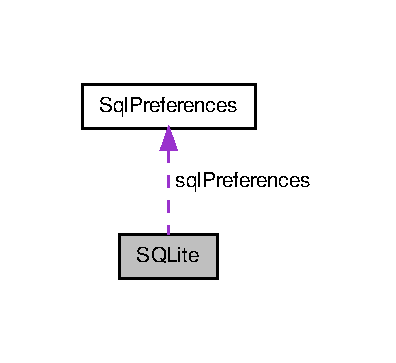
\includegraphics[width=190pt]{classSQLite__coll__graph}
\end{center}
\end{figure}
\subsection*{\-Public \-Member \-Functions}
\begin{DoxyCompactItemize}
\item 
\hyperlink{classSQLite_ae7b35dc7e3c41543a0acde669ad4ba0d}{\-S\-Q\-Lite} ()
\item 
void \hyperlink{classSQLite_ad04b99dcc053d1ad1fe034a7d33ddc45}{start\-Driver} (void)
\item 
void \hyperlink{classSQLite_a84d9c5795ea328449772de77bfd9e30e}{db\-Open} (void)
\item 
void \hyperlink{classSQLite_a846367e96132826f56b96515a2c1d8ab}{db\-Close} (void)
\item 
void \hyperlink{classSQLite_a245861da7b78b4adb356e552bd3b2286}{db\-Flush} (void)
\item 
bool \hyperlink{classSQLite_acd343255f8010fdde87b1d8b2cd65e49}{update\-D\-B\-Record} (\-Q\-String\-List data)
\item 
bool \hyperlink{classSQLite_aa4a76c8a9ec7d8a0101a28c228701e4b}{insert\-D\-B\-Record} (\-Q\-String\-List data)
\item 
bool \hyperlink{classSQLite_ae740e848da37fb08e92d2e7db3b508b7}{delete\-D\-B\-Record} ()
\item 
\-Q\-String\-List \hyperlink{classSQLite_a7c04908029911f3df653b673b3ee6e84}{select\-D\-B\-Record} (\-Q\-String start\-Idx)
\end{DoxyCompactItemize}
\subsection*{\-Public \-Attributes}
\begin{DoxyCompactItemize}
\item 
\-Q\-Sql\-Database \hyperlink{classSQLite_a1e719c7ea443e641471da642dbf33a70}{db}
\item 
\hyperlink{structSqlPreferences}{\-Sql\-Preferences} $\ast$ \hyperlink{classSQLite_a2dd6672e754497ad5ad90470e3ef3e33}{sql\-Preferences}
\end{DoxyCompactItemize}


\subsection{\-Detailed \-Description}


\-Definition at line 74 of file sqlite.\-h.



\subsection{\-Constructor \& \-Destructor \-Documentation}
\hypertarget{classSQLite_ae7b35dc7e3c41543a0acde669ad4ba0d}{\index{\-S\-Q\-Lite@{\-S\-Q\-Lite}!\-S\-Q\-Lite@{\-S\-Q\-Lite}}
\index{\-S\-Q\-Lite@{\-S\-Q\-Lite}!SQLite@{\-S\-Q\-Lite}}
\subsubsection[{\-S\-Q\-Lite}]{\setlength{\rightskip}{0pt plus 5cm}{\bf \-S\-Q\-Lite\-::\-S\-Q\-Lite} (
\begin{DoxyParamCaption}
{}
\end{DoxyParamCaption}
)}}\label{classSQLite_ae7b35dc7e3c41543a0acde669ad4ba0d}


\-Definition at line 42 of file sqlite.\-cpp.



\subsection{\-Member \-Function \-Documentation}
\hypertarget{classSQLite_a846367e96132826f56b96515a2c1d8ab}{\index{\-S\-Q\-Lite@{\-S\-Q\-Lite}!db\-Close@{db\-Close}}
\index{db\-Close@{db\-Close}!SQLite@{\-S\-Q\-Lite}}
\subsubsection[{db\-Close}]{\setlength{\rightskip}{0pt plus 5cm}void {\bf \-S\-Q\-Lite\-::db\-Close} (
\begin{DoxyParamCaption}
\item[{void}]{}
\end{DoxyParamCaption}
)}}\label{classSQLite_a846367e96132826f56b96515a2c1d8ab}


\-Definition at line 161 of file sqlite.\-cpp.

\hypertarget{classSQLite_a245861da7b78b4adb356e552bd3b2286}{\index{\-S\-Q\-Lite@{\-S\-Q\-Lite}!db\-Flush@{db\-Flush}}
\index{db\-Flush@{db\-Flush}!SQLite@{\-S\-Q\-Lite}}
\subsubsection[{db\-Flush}]{\setlength{\rightskip}{0pt plus 5cm}void {\bf \-S\-Q\-Lite\-::db\-Flush} (
\begin{DoxyParamCaption}
\item[{void}]{}
\end{DoxyParamCaption}
)}}\label{classSQLite_a245861da7b78b4adb356e552bd3b2286}


\-Definition at line 156 of file sqlite.\-cpp.



\-Here is the caller graph for this function\-:\nopagebreak
\begin{figure}[H]
\begin{center}
\leavevmode
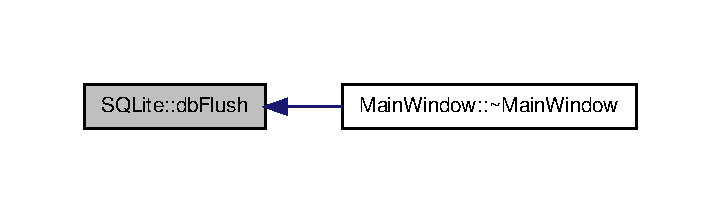
\includegraphics[width=346pt]{classSQLite_a245861da7b78b4adb356e552bd3b2286_icgraph}
\end{center}
\end{figure}


\hypertarget{classSQLite_a84d9c5795ea328449772de77bfd9e30e}{\index{\-S\-Q\-Lite@{\-S\-Q\-Lite}!db\-Open@{db\-Open}}
\index{db\-Open@{db\-Open}!SQLite@{\-S\-Q\-Lite}}
\subsubsection[{db\-Open}]{\setlength{\rightskip}{0pt plus 5cm}void {\bf \-S\-Q\-Lite\-::db\-Open} (
\begin{DoxyParamCaption}
\item[{void}]{}
\end{DoxyParamCaption}
)}}\label{classSQLite_a84d9c5795ea328449772de77bfd9e30e}


\-Definition at line 167 of file sqlite.\-cpp.

\hypertarget{classSQLite_ae740e848da37fb08e92d2e7db3b508b7}{\index{\-S\-Q\-Lite@{\-S\-Q\-Lite}!delete\-D\-B\-Record@{delete\-D\-B\-Record}}
\index{delete\-D\-B\-Record@{delete\-D\-B\-Record}!SQLite@{\-S\-Q\-Lite}}
\subsubsection[{delete\-D\-B\-Record}]{\setlength{\rightskip}{0pt plus 5cm}bool {\bf \-S\-Q\-Lite\-::delete\-D\-B\-Record} (
\begin{DoxyParamCaption}
{}
\end{DoxyParamCaption}
)}}\label{classSQLite_ae740e848da37fb08e92d2e7db3b508b7}


\-Definition at line 211 of file sqlite.\-cpp.

\hypertarget{classSQLite_aa4a76c8a9ec7d8a0101a28c228701e4b}{\index{\-S\-Q\-Lite@{\-S\-Q\-Lite}!insert\-D\-B\-Record@{insert\-D\-B\-Record}}
\index{insert\-D\-B\-Record@{insert\-D\-B\-Record}!SQLite@{\-S\-Q\-Lite}}
\subsubsection[{insert\-D\-B\-Record}]{\setlength{\rightskip}{0pt plus 5cm}bool {\bf \-S\-Q\-Lite\-::insert\-D\-B\-Record} (
\begin{DoxyParamCaption}
\item[{\-Q\-String\-List}]{data}
\end{DoxyParamCaption}
)}}\label{classSQLite_aa4a76c8a9ec7d8a0101a28c228701e4b}


\-Definition at line 194 of file sqlite.\-cpp.

\hypertarget{classSQLite_a7c04908029911f3df653b673b3ee6e84}{\index{\-S\-Q\-Lite@{\-S\-Q\-Lite}!select\-D\-B\-Record@{select\-D\-B\-Record}}
\index{select\-D\-B\-Record@{select\-D\-B\-Record}!SQLite@{\-S\-Q\-Lite}}
\subsubsection[{select\-D\-B\-Record}]{\setlength{\rightskip}{0pt plus 5cm}\-Q\-String\-List {\bf \-S\-Q\-Lite\-::select\-D\-B\-Record} (
\begin{DoxyParamCaption}
\item[{\-Q\-String}]{start\-Idx}
\end{DoxyParamCaption}
)}}\label{classSQLite_a7c04908029911f3df653b673b3ee6e84}


\-Definition at line 218 of file sqlite.\-cpp.

\hypertarget{classSQLite_ad04b99dcc053d1ad1fe034a7d33ddc45}{\index{\-S\-Q\-Lite@{\-S\-Q\-Lite}!start\-Driver@{start\-Driver}}
\index{start\-Driver@{start\-Driver}!SQLite@{\-S\-Q\-Lite}}
\subsubsection[{start\-Driver}]{\setlength{\rightskip}{0pt plus 5cm}void {\bf \-S\-Q\-Lite\-::start\-Driver} (
\begin{DoxyParamCaption}
\item[{void}]{}
\end{DoxyParamCaption}
)}}\label{classSQLite_ad04b99dcc053d1ad1fe034a7d33ddc45}


\-Definition at line 46 of file sqlite.\-cpp.



\-Here is the caller graph for this function\-:\nopagebreak
\begin{figure}[H]
\begin{center}
\leavevmode
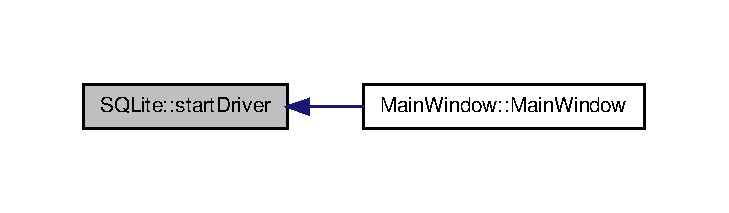
\includegraphics[width=350pt]{classSQLite_ad04b99dcc053d1ad1fe034a7d33ddc45_icgraph}
\end{center}
\end{figure}


\hypertarget{classSQLite_acd343255f8010fdde87b1d8b2cd65e49}{\index{\-S\-Q\-Lite@{\-S\-Q\-Lite}!update\-D\-B\-Record@{update\-D\-B\-Record}}
\index{update\-D\-B\-Record@{update\-D\-B\-Record}!SQLite@{\-S\-Q\-Lite}}
\subsubsection[{update\-D\-B\-Record}]{\setlength{\rightskip}{0pt plus 5cm}bool {\bf \-S\-Q\-Lite\-::update\-D\-B\-Record} (
\begin{DoxyParamCaption}
\item[{\-Q\-String\-List}]{data}
\end{DoxyParamCaption}
)}}\label{classSQLite_acd343255f8010fdde87b1d8b2cd65e49}


\-Definition at line 176 of file sqlite.\-cpp.



\subsection{\-Member \-Data \-Documentation}
\hypertarget{classSQLite_a1e719c7ea443e641471da642dbf33a70}{\index{\-S\-Q\-Lite@{\-S\-Q\-Lite}!db@{db}}
\index{db@{db}!SQLite@{\-S\-Q\-Lite}}
\subsubsection[{db}]{\setlength{\rightskip}{0pt plus 5cm}\-Q\-Sql\-Database {\bf \-S\-Q\-Lite\-::db}}}\label{classSQLite_a1e719c7ea443e641471da642dbf33a70}


\-Definition at line 87 of file sqlite.\-h.

\hypertarget{classSQLite_a2dd6672e754497ad5ad90470e3ef3e33}{\index{\-S\-Q\-Lite@{\-S\-Q\-Lite}!sql\-Preferences@{sql\-Preferences}}
\index{sql\-Preferences@{sql\-Preferences}!SQLite@{\-S\-Q\-Lite}}
\subsubsection[{sql\-Preferences}]{\setlength{\rightskip}{0pt plus 5cm}{\bf \-Sql\-Preferences}$\ast$ {\bf \-S\-Q\-Lite\-::sql\-Preferences}}}\label{classSQLite_a2dd6672e754497ad5ad90470e3ef3e33}


\-Definition at line 88 of file sqlite.\-h.



\-The documentation for this class was generated from the following files\-:\begin{DoxyCompactItemize}
\item 
\hyperlink{sqlite_8h}{sqlite.\-h}\item 
\hyperlink{sqlite_8cpp}{sqlite.\-cpp}\end{DoxyCompactItemize}

\hypertarget{structSqlPreferences}{\section{\-Sql\-Preferences \-Struct \-Reference}
\label{structSqlPreferences}\index{\-Sql\-Preferences@{\-Sql\-Preferences}}
}


{\ttfamily \#include $<$sqlite.\-h$>$}

\subsection*{\-Public \-Attributes}
\begin{DoxyCompactItemize}
\item 
bool \hyperlink{structSqlPreferences_a36464d4021afe0e0919cce650a1519fe}{use\-Atomic\-Commit}
\item 
bool \hyperlink{structSqlPreferences_a7e53d4abaf46acfb84cd8c30fbf3b1df}{use\-Custom\-Page\-Size}
\item 
bool \hyperlink{structSqlPreferences_ad26f9920ddc5ac5f655873d9ecb3ac53}{use\-Custom\-Cache\-Size}
\item 
bool \hyperlink{structSqlPreferences_abcd9f162cf432b71159c7c83adb8ac88}{use\-Custom\-Temp\-Store}
\item 
bool \hyperlink{structSqlPreferences_a9aa98cdd591864c7b2382b2d0fff0de9}{use\-Custom\-Journal\-Mode}
\item 
bool \hyperlink{structSqlPreferences_a22c08a63c97db2f85e08920bf3e22516}{use\-Custom\-Locking\-Mode}
\item 
bool \hyperlink{structSqlPreferences_a3d18d11573e0546e8fe854b7584adab7}{use\-Custom\-Synchronous}
\item 
bool \hyperlink{structSqlPreferences_ae8bb4bc0c82e4f32c51efdbf3d3e1af5}{use\-Exist\-D\-B}
\item 
bool \hyperlink{structSqlPreferences_ad7d06ce81f298cf13b7522e48d640a78}{use\-Ram\-D\-B}
\item 
\-Q\-String \hyperlink{structSqlPreferences_aeaa6fa937ead293aa8cd41b86f1c5cf4}{custom\-Page\-Size}
\item 
\-Q\-String \hyperlink{structSqlPreferences_a623f8f8b12bdde7ce2c69f6388d3719b}{custom\-Cache\-Size}
\item 
\-Q\-String \hyperlink{structSqlPreferences_a36b942f872c390f204cc5542fc0662de}{custom\-Temp\-Store}
\item 
\-Q\-String \hyperlink{structSqlPreferences_afa1cee8e11c7ca38d32e05c92a6b56da}{custom\-Journal\-Mode}
\item 
\-Q\-String \hyperlink{structSqlPreferences_ad99a3e0cc0c19283aa9337e6a28f0a28}{custom\-Locking\-Mode}
\item 
\-Q\-String \hyperlink{structSqlPreferences_a7d309904c4edb9f888d0c8a810def2d1}{custom\-Synchronous}
\end{DoxyCompactItemize}


\subsection{\-Detailed \-Description}


\-Definition at line 54 of file sqlite.\-h.



\subsection{\-Member \-Data \-Documentation}
\hypertarget{structSqlPreferences_a623f8f8b12bdde7ce2c69f6388d3719b}{\index{\-Sql\-Preferences@{\-Sql\-Preferences}!custom\-Cache\-Size@{custom\-Cache\-Size}}
\index{custom\-Cache\-Size@{custom\-Cache\-Size}!SqlPreferences@{\-Sql\-Preferences}}
\subsubsection[{custom\-Cache\-Size}]{\setlength{\rightskip}{0pt plus 5cm}\-Q\-String {\bf \-Sql\-Preferences\-::custom\-Cache\-Size}}}\label{structSqlPreferences_a623f8f8b12bdde7ce2c69f6388d3719b}


\-Definition at line 66 of file sqlite.\-h.

\hypertarget{structSqlPreferences_afa1cee8e11c7ca38d32e05c92a6b56da}{\index{\-Sql\-Preferences@{\-Sql\-Preferences}!custom\-Journal\-Mode@{custom\-Journal\-Mode}}
\index{custom\-Journal\-Mode@{custom\-Journal\-Mode}!SqlPreferences@{\-Sql\-Preferences}}
\subsubsection[{custom\-Journal\-Mode}]{\setlength{\rightskip}{0pt plus 5cm}\-Q\-String {\bf \-Sql\-Preferences\-::custom\-Journal\-Mode}}}\label{structSqlPreferences_afa1cee8e11c7ca38d32e05c92a6b56da}


\-Definition at line 68 of file sqlite.\-h.

\hypertarget{structSqlPreferences_ad99a3e0cc0c19283aa9337e6a28f0a28}{\index{\-Sql\-Preferences@{\-Sql\-Preferences}!custom\-Locking\-Mode@{custom\-Locking\-Mode}}
\index{custom\-Locking\-Mode@{custom\-Locking\-Mode}!SqlPreferences@{\-Sql\-Preferences}}
\subsubsection[{custom\-Locking\-Mode}]{\setlength{\rightskip}{0pt plus 5cm}\-Q\-String {\bf \-Sql\-Preferences\-::custom\-Locking\-Mode}}}\label{structSqlPreferences_ad99a3e0cc0c19283aa9337e6a28f0a28}


\-Definition at line 69 of file sqlite.\-h.

\hypertarget{structSqlPreferences_aeaa6fa937ead293aa8cd41b86f1c5cf4}{\index{\-Sql\-Preferences@{\-Sql\-Preferences}!custom\-Page\-Size@{custom\-Page\-Size}}
\index{custom\-Page\-Size@{custom\-Page\-Size}!SqlPreferences@{\-Sql\-Preferences}}
\subsubsection[{custom\-Page\-Size}]{\setlength{\rightskip}{0pt plus 5cm}\-Q\-String {\bf \-Sql\-Preferences\-::custom\-Page\-Size}}}\label{structSqlPreferences_aeaa6fa937ead293aa8cd41b86f1c5cf4}


\-Definition at line 65 of file sqlite.\-h.

\hypertarget{structSqlPreferences_a7d309904c4edb9f888d0c8a810def2d1}{\index{\-Sql\-Preferences@{\-Sql\-Preferences}!custom\-Synchronous@{custom\-Synchronous}}
\index{custom\-Synchronous@{custom\-Synchronous}!SqlPreferences@{\-Sql\-Preferences}}
\subsubsection[{custom\-Synchronous}]{\setlength{\rightskip}{0pt plus 5cm}\-Q\-String {\bf \-Sql\-Preferences\-::custom\-Synchronous}}}\label{structSqlPreferences_a7d309904c4edb9f888d0c8a810def2d1}


\-Definition at line 70 of file sqlite.\-h.

\hypertarget{structSqlPreferences_a36b942f872c390f204cc5542fc0662de}{\index{\-Sql\-Preferences@{\-Sql\-Preferences}!custom\-Temp\-Store@{custom\-Temp\-Store}}
\index{custom\-Temp\-Store@{custom\-Temp\-Store}!SqlPreferences@{\-Sql\-Preferences}}
\subsubsection[{custom\-Temp\-Store}]{\setlength{\rightskip}{0pt plus 5cm}\-Q\-String {\bf \-Sql\-Preferences\-::custom\-Temp\-Store}}}\label{structSqlPreferences_a36b942f872c390f204cc5542fc0662de}


\-Definition at line 67 of file sqlite.\-h.

\hypertarget{structSqlPreferences_a36464d4021afe0e0919cce650a1519fe}{\index{\-Sql\-Preferences@{\-Sql\-Preferences}!use\-Atomic\-Commit@{use\-Atomic\-Commit}}
\index{use\-Atomic\-Commit@{use\-Atomic\-Commit}!SqlPreferences@{\-Sql\-Preferences}}
\subsubsection[{use\-Atomic\-Commit}]{\setlength{\rightskip}{0pt plus 5cm}bool {\bf \-Sql\-Preferences\-::use\-Atomic\-Commit}}}\label{structSqlPreferences_a36464d4021afe0e0919cce650a1519fe}


\-Definition at line 56 of file sqlite.\-h.

\hypertarget{structSqlPreferences_ad26f9920ddc5ac5f655873d9ecb3ac53}{\index{\-Sql\-Preferences@{\-Sql\-Preferences}!use\-Custom\-Cache\-Size@{use\-Custom\-Cache\-Size}}
\index{use\-Custom\-Cache\-Size@{use\-Custom\-Cache\-Size}!SqlPreferences@{\-Sql\-Preferences}}
\subsubsection[{use\-Custom\-Cache\-Size}]{\setlength{\rightskip}{0pt plus 5cm}bool {\bf \-Sql\-Preferences\-::use\-Custom\-Cache\-Size}}}\label{structSqlPreferences_ad26f9920ddc5ac5f655873d9ecb3ac53}


\-Definition at line 58 of file sqlite.\-h.

\hypertarget{structSqlPreferences_a9aa98cdd591864c7b2382b2d0fff0de9}{\index{\-Sql\-Preferences@{\-Sql\-Preferences}!use\-Custom\-Journal\-Mode@{use\-Custom\-Journal\-Mode}}
\index{use\-Custom\-Journal\-Mode@{use\-Custom\-Journal\-Mode}!SqlPreferences@{\-Sql\-Preferences}}
\subsubsection[{use\-Custom\-Journal\-Mode}]{\setlength{\rightskip}{0pt plus 5cm}bool {\bf \-Sql\-Preferences\-::use\-Custom\-Journal\-Mode}}}\label{structSqlPreferences_a9aa98cdd591864c7b2382b2d0fff0de9}


\-Definition at line 60 of file sqlite.\-h.

\hypertarget{structSqlPreferences_a22c08a63c97db2f85e08920bf3e22516}{\index{\-Sql\-Preferences@{\-Sql\-Preferences}!use\-Custom\-Locking\-Mode@{use\-Custom\-Locking\-Mode}}
\index{use\-Custom\-Locking\-Mode@{use\-Custom\-Locking\-Mode}!SqlPreferences@{\-Sql\-Preferences}}
\subsubsection[{use\-Custom\-Locking\-Mode}]{\setlength{\rightskip}{0pt plus 5cm}bool {\bf \-Sql\-Preferences\-::use\-Custom\-Locking\-Mode}}}\label{structSqlPreferences_a22c08a63c97db2f85e08920bf3e22516}


\-Definition at line 61 of file sqlite.\-h.

\hypertarget{structSqlPreferences_a7e53d4abaf46acfb84cd8c30fbf3b1df}{\index{\-Sql\-Preferences@{\-Sql\-Preferences}!use\-Custom\-Page\-Size@{use\-Custom\-Page\-Size}}
\index{use\-Custom\-Page\-Size@{use\-Custom\-Page\-Size}!SqlPreferences@{\-Sql\-Preferences}}
\subsubsection[{use\-Custom\-Page\-Size}]{\setlength{\rightskip}{0pt plus 5cm}bool {\bf \-Sql\-Preferences\-::use\-Custom\-Page\-Size}}}\label{structSqlPreferences_a7e53d4abaf46acfb84cd8c30fbf3b1df}


\-Definition at line 57 of file sqlite.\-h.

\hypertarget{structSqlPreferences_a3d18d11573e0546e8fe854b7584adab7}{\index{\-Sql\-Preferences@{\-Sql\-Preferences}!use\-Custom\-Synchronous@{use\-Custom\-Synchronous}}
\index{use\-Custom\-Synchronous@{use\-Custom\-Synchronous}!SqlPreferences@{\-Sql\-Preferences}}
\subsubsection[{use\-Custom\-Synchronous}]{\setlength{\rightskip}{0pt plus 5cm}bool {\bf \-Sql\-Preferences\-::use\-Custom\-Synchronous}}}\label{structSqlPreferences_a3d18d11573e0546e8fe854b7584adab7}


\-Definition at line 62 of file sqlite.\-h.

\hypertarget{structSqlPreferences_abcd9f162cf432b71159c7c83adb8ac88}{\index{\-Sql\-Preferences@{\-Sql\-Preferences}!use\-Custom\-Temp\-Store@{use\-Custom\-Temp\-Store}}
\index{use\-Custom\-Temp\-Store@{use\-Custom\-Temp\-Store}!SqlPreferences@{\-Sql\-Preferences}}
\subsubsection[{use\-Custom\-Temp\-Store}]{\setlength{\rightskip}{0pt plus 5cm}bool {\bf \-Sql\-Preferences\-::use\-Custom\-Temp\-Store}}}\label{structSqlPreferences_abcd9f162cf432b71159c7c83adb8ac88}


\-Definition at line 59 of file sqlite.\-h.

\hypertarget{structSqlPreferences_ae8bb4bc0c82e4f32c51efdbf3d3e1af5}{\index{\-Sql\-Preferences@{\-Sql\-Preferences}!use\-Exist\-D\-B@{use\-Exist\-D\-B}}
\index{use\-Exist\-D\-B@{use\-Exist\-D\-B}!SqlPreferences@{\-Sql\-Preferences}}
\subsubsection[{use\-Exist\-D\-B}]{\setlength{\rightskip}{0pt plus 5cm}bool {\bf \-Sql\-Preferences\-::use\-Exist\-D\-B}}}\label{structSqlPreferences_ae8bb4bc0c82e4f32c51efdbf3d3e1af5}


\-Definition at line 63 of file sqlite.\-h.

\hypertarget{structSqlPreferences_ad7d06ce81f298cf13b7522e48d640a78}{\index{\-Sql\-Preferences@{\-Sql\-Preferences}!use\-Ram\-D\-B@{use\-Ram\-D\-B}}
\index{use\-Ram\-D\-B@{use\-Ram\-D\-B}!SqlPreferences@{\-Sql\-Preferences}}
\subsubsection[{use\-Ram\-D\-B}]{\setlength{\rightskip}{0pt plus 5cm}bool {\bf \-Sql\-Preferences\-::use\-Ram\-D\-B}}}\label{structSqlPreferences_ad7d06ce81f298cf13b7522e48d640a78}


\-Definition at line 64 of file sqlite.\-h.



\-The documentation for this struct was generated from the following file\-:\begin{DoxyCompactItemize}
\item 
\hyperlink{sqlite_8h}{sqlite.\-h}\end{DoxyCompactItemize}

\chapter{\-File \-Documentation}
\hypertarget{aboutdialog_8cpp}{\section{aboutdialog.\-cpp \-File \-Reference}
\label{aboutdialog_8cpp}\index{aboutdialog.\-cpp@{aboutdialog.\-cpp}}
}
{\ttfamily \#include \char`\"{}aboutdialog.\-h\char`\"{}}\*
{\ttfamily \#include \char`\"{}ui\-\_\-aboutdialog.\-h\char`\"{}}\*
\-Include dependency graph for aboutdialog.\-cpp\-:\nopagebreak
\begin{figure}[H]
\begin{center}
\leavevmode
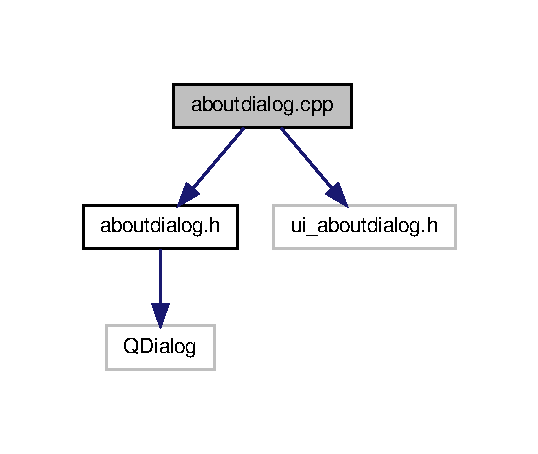
\includegraphics[width=258pt]{aboutdialog_8cpp__incl}
\end{center}
\end{figure}
\subsection*{\-Namespaces}
\begin{DoxyCompactItemize}
\item 
namespace \hyperlink{namespacesqlitetest}{sqlitetest}
\end{DoxyCompactItemize}

\hypertarget{aboutdialog_8h}{\section{aboutdialog.\-h \-File \-Reference}
\label{aboutdialog_8h}\index{aboutdialog.\-h@{aboutdialog.\-h}}
}
{\ttfamily \#include $<$\-Q\-Dialog$>$}\*
\-Include dependency graph for aboutdialog.\-h\-:\nopagebreak
\begin{figure}[H]
\begin{center}
\leavevmode
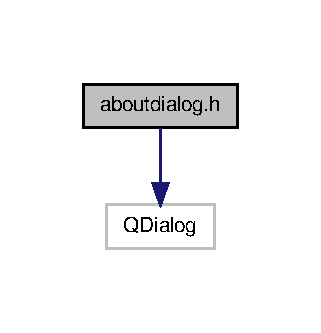
\includegraphics[width=154pt]{aboutdialog_8h__incl}
\end{center}
\end{figure}
\-This graph shows which files directly or indirectly include this file\-:\nopagebreak
\begin{figure}[H]
\begin{center}
\leavevmode
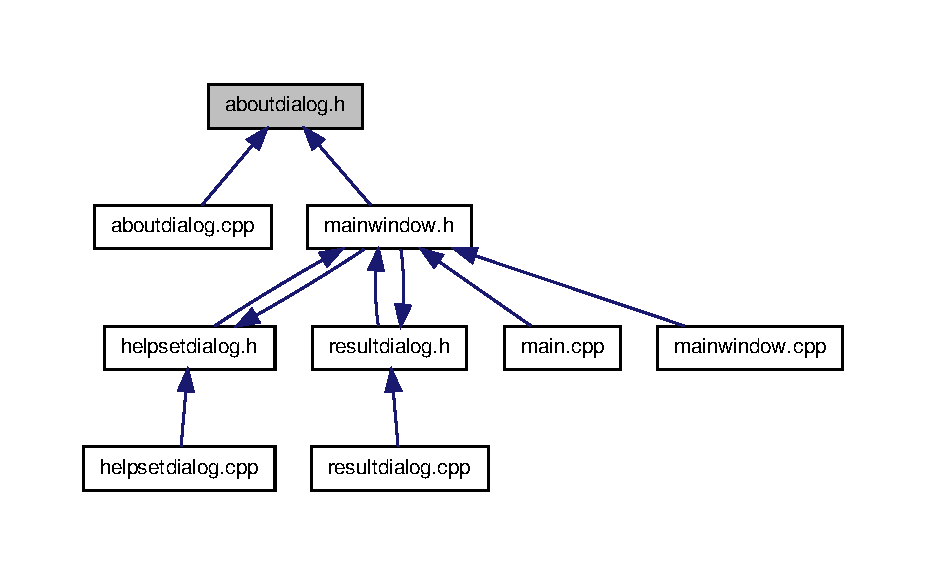
\includegraphics[width=350pt]{aboutdialog_8h__dep__incl}
\end{center}
\end{figure}
\subsection*{\-Classes}
\begin{DoxyCompactItemize}
\item 
class \hyperlink{classAboutDialog}{\-About\-Dialog}
\end{DoxyCompactItemize}
\subsection*{\-Namespaces}
\begin{DoxyCompactItemize}
\item 
namespace \hyperlink{namespacesqlitetest}{sqlitetest}
\item 
namespace \hyperlink{namespaceUi}{\-Ui}
\end{DoxyCompactItemize}

\hypertarget{helpsetdialog_8cpp}{\section{helpsetdialog.\-cpp \-File \-Reference}
\label{helpsetdialog_8cpp}\index{helpsetdialog.\-cpp@{helpsetdialog.\-cpp}}
}
{\ttfamily \#include \char`\"{}helpsetdialog.\-h\char`\"{}}\*
{\ttfamily \#include \char`\"{}ui\-\_\-helpsetdialog.\-h\char`\"{}}\*
\-Include dependency graph for helpsetdialog.\-cpp\-:\nopagebreak
\begin{figure}[H]
\begin{center}
\leavevmode
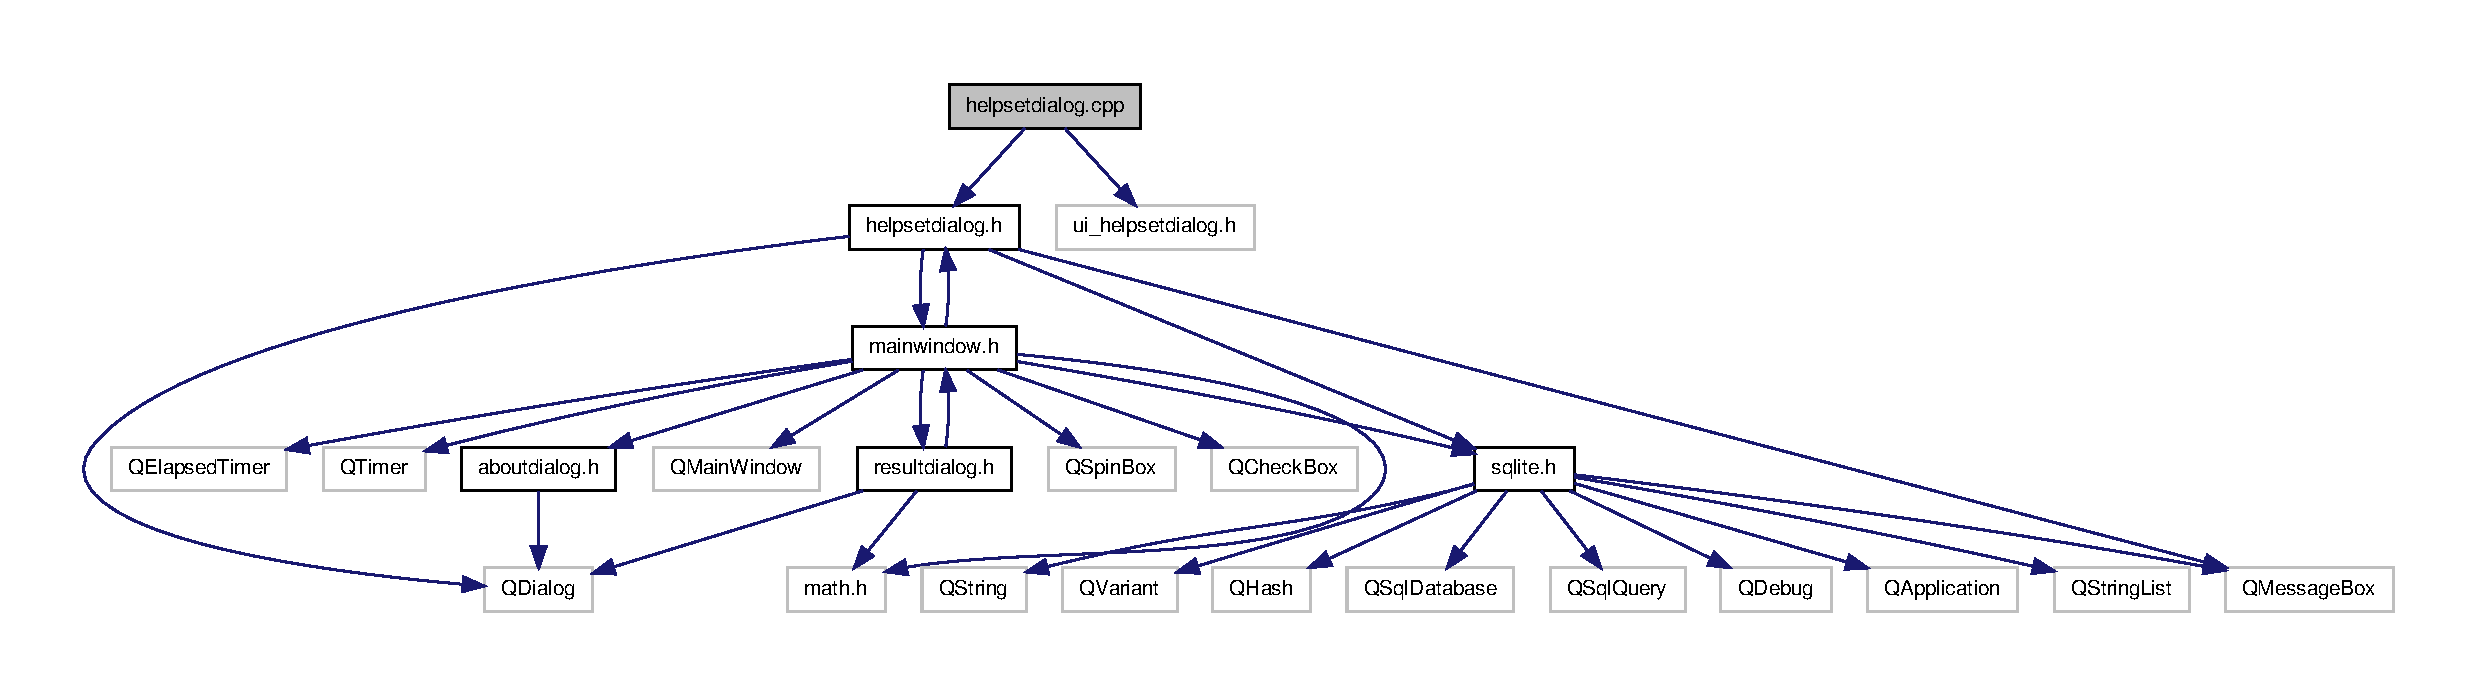
\includegraphics[width=350pt]{helpsetdialog_8cpp__incl}
\end{center}
\end{figure}
\subsection*{\-Namespaces}
\begin{DoxyCompactItemize}
\item 
namespace \hyperlink{namespacesqlitetest}{sqlitetest}
\end{DoxyCompactItemize}

\hypertarget{helpsetdialog_8h}{\section{helpsetdialog.\-h \-File \-Reference}
\label{helpsetdialog_8h}\index{helpsetdialog.\-h@{helpsetdialog.\-h}}
}
{\ttfamily \#include $<$\-Q\-Dialog$>$}\*
{\ttfamily \#include $<$\-Q\-Message\-Box$>$}\*
{\ttfamily \#include \char`\"{}mainwindow.\-h\char`\"{}}\*
{\ttfamily \#include \char`\"{}sqlite.\-h\char`\"{}}\*
\-Include dependency graph for helpsetdialog.\-h\-:\nopagebreak
\begin{figure}[H]
\begin{center}
\leavevmode
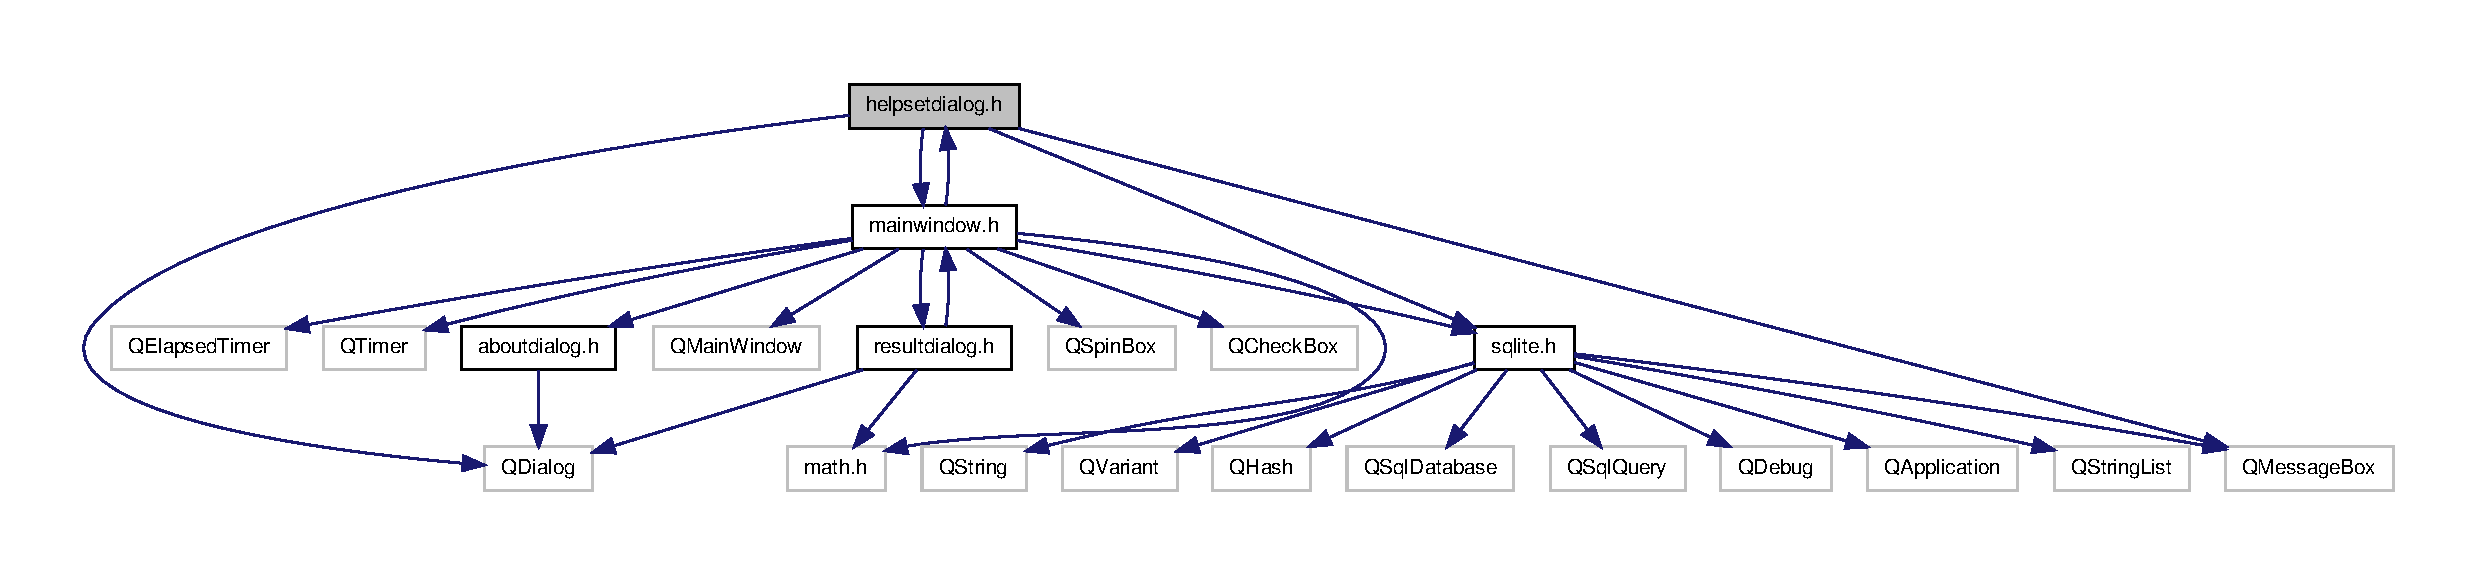
\includegraphics[width=350pt]{helpsetdialog_8h__incl}
\end{center}
\end{figure}
\-This graph shows which files directly or indirectly include this file\-:\nopagebreak
\begin{figure}[H]
\begin{center}
\leavevmode
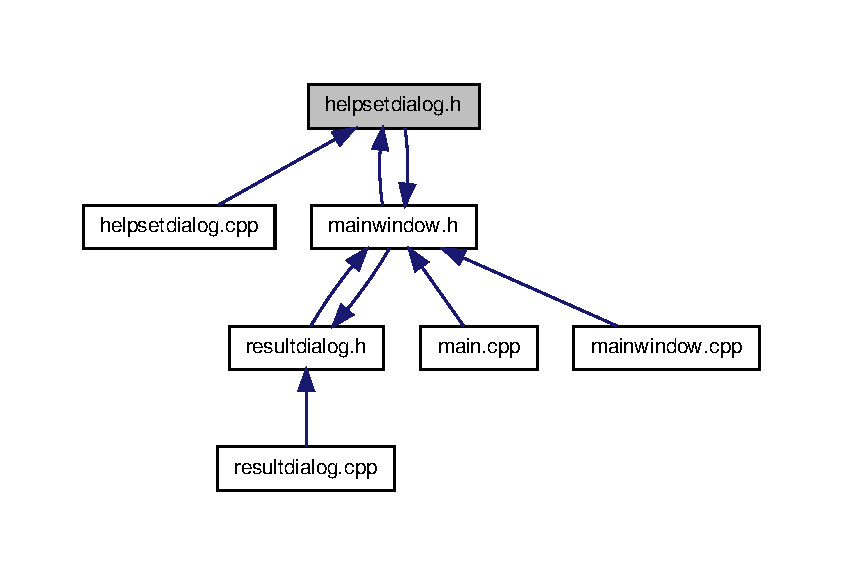
\includegraphics[width=350pt]{helpsetdialog_8h__dep__incl}
\end{center}
\end{figure}
\subsection*{\-Classes}
\begin{DoxyCompactItemize}
\item 
class \hyperlink{classHelpSetDialog}{\-Help\-Set\-Dialog}
\end{DoxyCompactItemize}
\subsection*{\-Namespaces}
\begin{DoxyCompactItemize}
\item 
namespace \hyperlink{namespacesqlitetest}{sqlitetest}
\item 
namespace \hyperlink{namespaceUi}{\-Ui}
\end{DoxyCompactItemize}

\hypertarget{main_8cpp}{\section{main.\-cpp \-File \-Reference}
\label{main_8cpp}\index{main.\-cpp@{main.\-cpp}}
}
{\ttfamily \#include $<$\-Qt\-Gui/\-Q\-Application$>$}\*
{\ttfamily \#include \char`\"{}mainwindow.\-h\char`\"{}}\*
\-Include dependency graph for main.\-cpp\-:\nopagebreak
\begin{figure}[H]
\begin{center}
\leavevmode
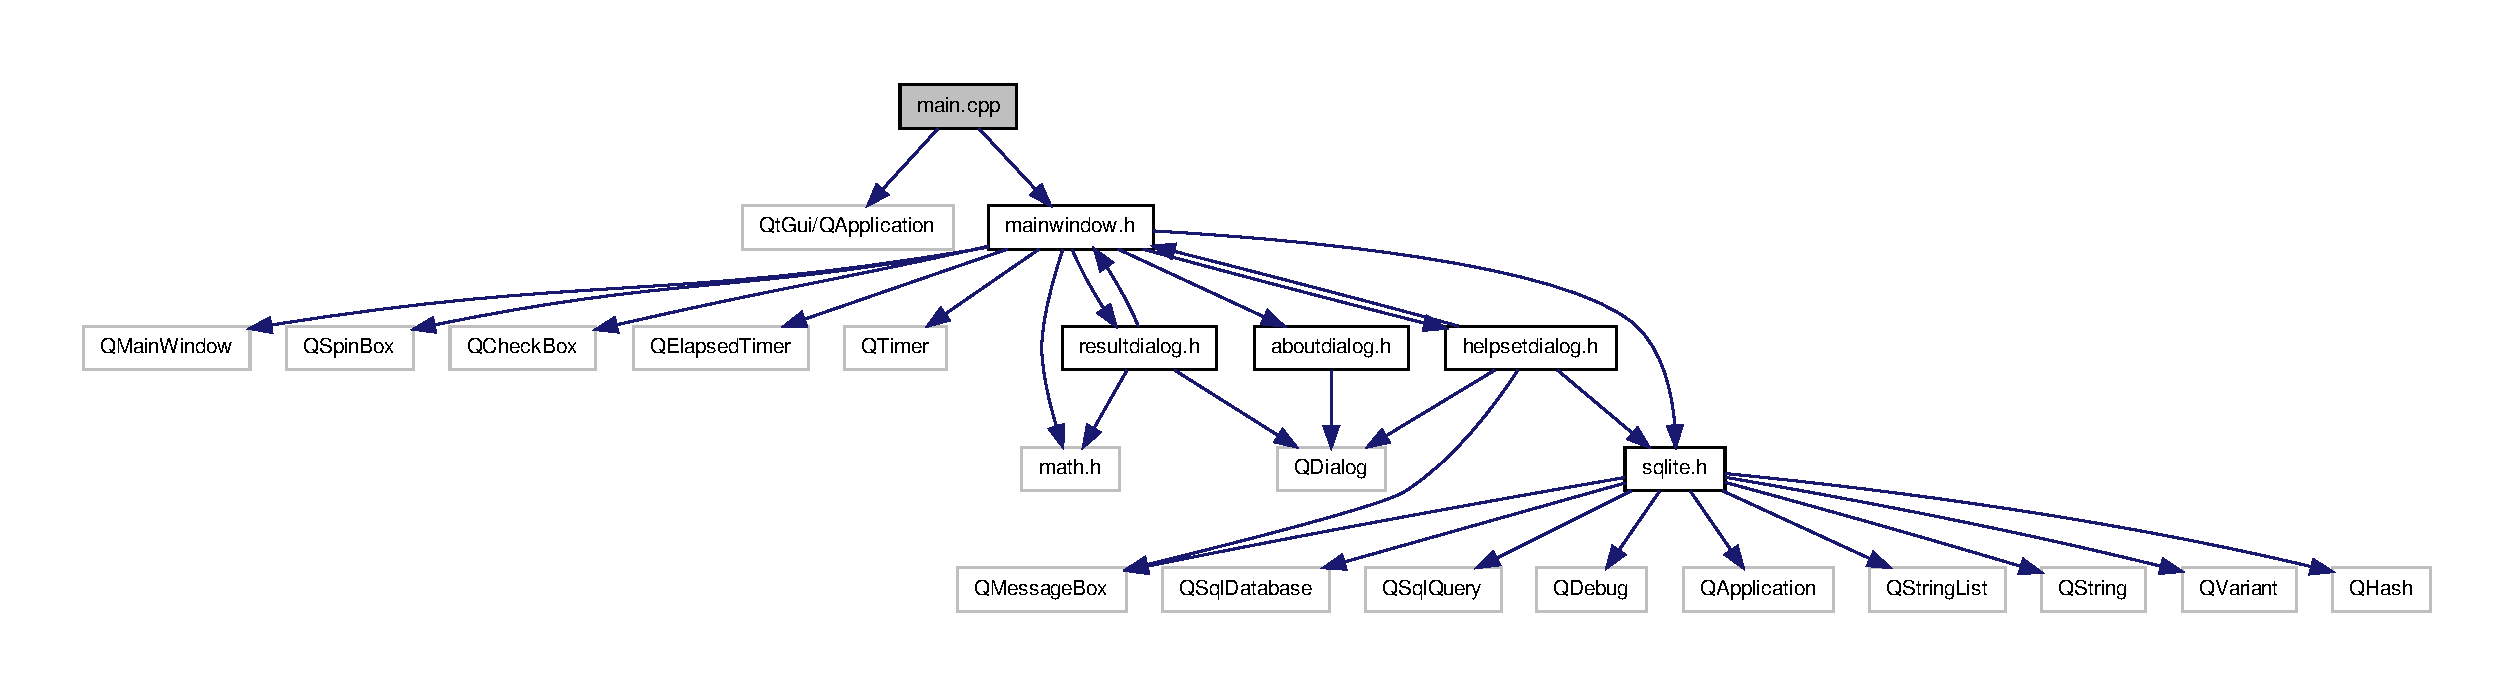
\includegraphics[width=350pt]{main_8cpp__incl}
\end{center}
\end{figure}
\subsection*{\-Namespaces}
\begin{DoxyCompactItemize}
\item 
namespace \hyperlink{namespacesqlitetest}{sqlitetest}
\end{DoxyCompactItemize}
\subsection*{\-Functions}
\begin{DoxyCompactItemize}
\item 
int \hyperlink{main_8cpp_a0ddf1224851353fc92bfbff6f499fa97}{main} (int argc, char $\ast$argv\mbox{[}$\,$\mbox{]})
\end{DoxyCompactItemize}


\subsection{\-Function \-Documentation}
\hypertarget{main_8cpp_a0ddf1224851353fc92bfbff6f499fa97}{\index{main.\-cpp@{main.\-cpp}!main@{main}}
\index{main@{main}!main.cpp@{main.\-cpp}}
\subsubsection[{main}]{\setlength{\rightskip}{0pt plus 5cm}int {\bf main} (
\begin{DoxyParamCaption}
\item[{int}]{argc, }
\item[{char $\ast$}]{argv\mbox{[}$\,$\mbox{]}}
\end{DoxyParamCaption}
)}}\label{main_8cpp_a0ddf1224851353fc92bfbff6f499fa97}


\-Definition at line 40 of file main.\-cpp.


\hypertarget{mainwindow_8cpp}{\section{mainwindow.\-cpp \-File \-Reference}
\label{mainwindow_8cpp}\index{mainwindow.\-cpp@{mainwindow.\-cpp}}
}
{\ttfamily \#include \char`\"{}mainwindow.\-h\char`\"{}}\*
{\ttfamily \#include \char`\"{}ui\-\_\-mainwindow.\-h\char`\"{}}\*
\-Include dependency graph for mainwindow.\-cpp\-:\nopagebreak
\begin{figure}[H]
\begin{center}
\leavevmode
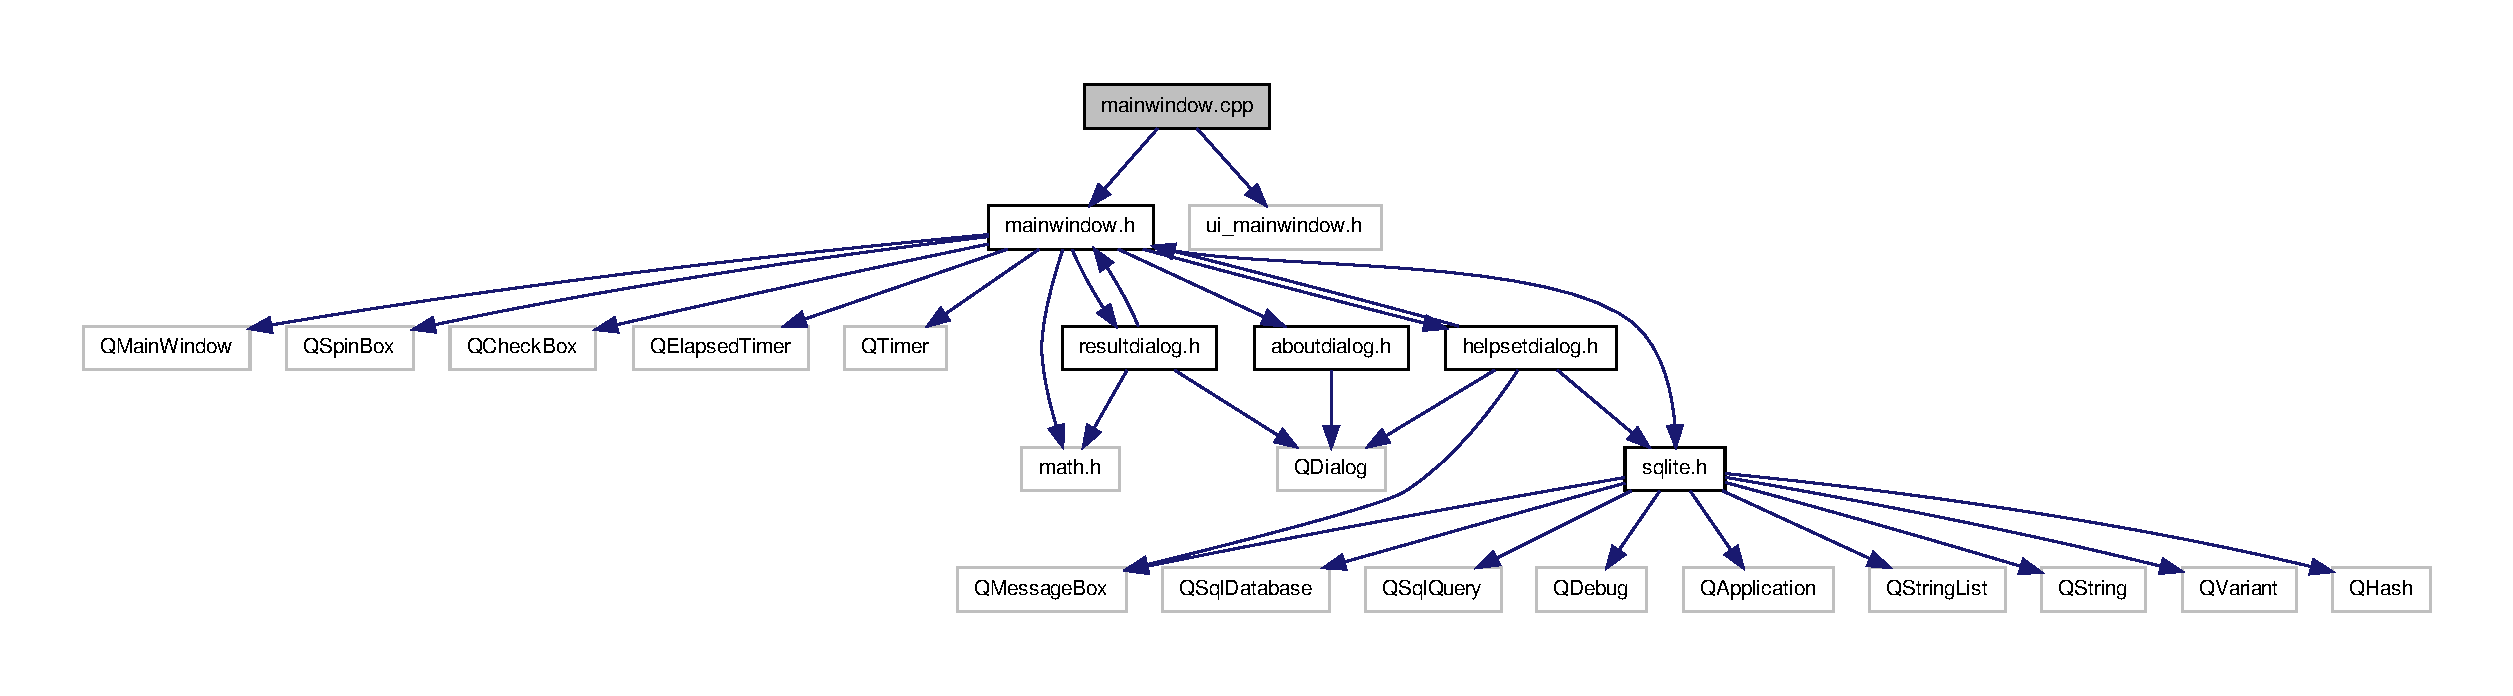
\includegraphics[width=350pt]{mainwindow_8cpp__incl}
\end{center}
\end{figure}
\subsection*{\-Namespaces}
\begin{DoxyCompactItemize}
\item 
namespace \hyperlink{namespacesqlitetest}{sqlitetest}
\end{DoxyCompactItemize}

\hypertarget{mainwindow_8h}{\section{mainwindow.\-h \-File \-Reference}
\label{mainwindow_8h}\index{mainwindow.\-h@{mainwindow.\-h}}
}
{\ttfamily \#include $<$\-Q\-Main\-Window$>$}\*
{\ttfamily \#include $<$\-Q\-Spin\-Box$>$}\*
{\ttfamily \#include $<$\-Q\-Check\-Box$>$}\*
{\ttfamily \#include $<$\-Q\-Elapsed\-Timer$>$}\*
{\ttfamily \#include $<$\-Q\-Timer$>$}\*
{\ttfamily \#include $<$math.\-h$>$}\*
{\ttfamily \#include \char`\"{}sqlite.\-h\char`\"{}}\*
{\ttfamily \#include \char`\"{}helpsetdialog.\-h\char`\"{}}\*
{\ttfamily \#include \char`\"{}aboutdialog.\-h\char`\"{}}\*
{\ttfamily \#include \char`\"{}resultdialog.\-h\char`\"{}}\*
\-Include dependency graph for mainwindow.\-h\-:\nopagebreak
\begin{figure}[H]
\begin{center}
\leavevmode
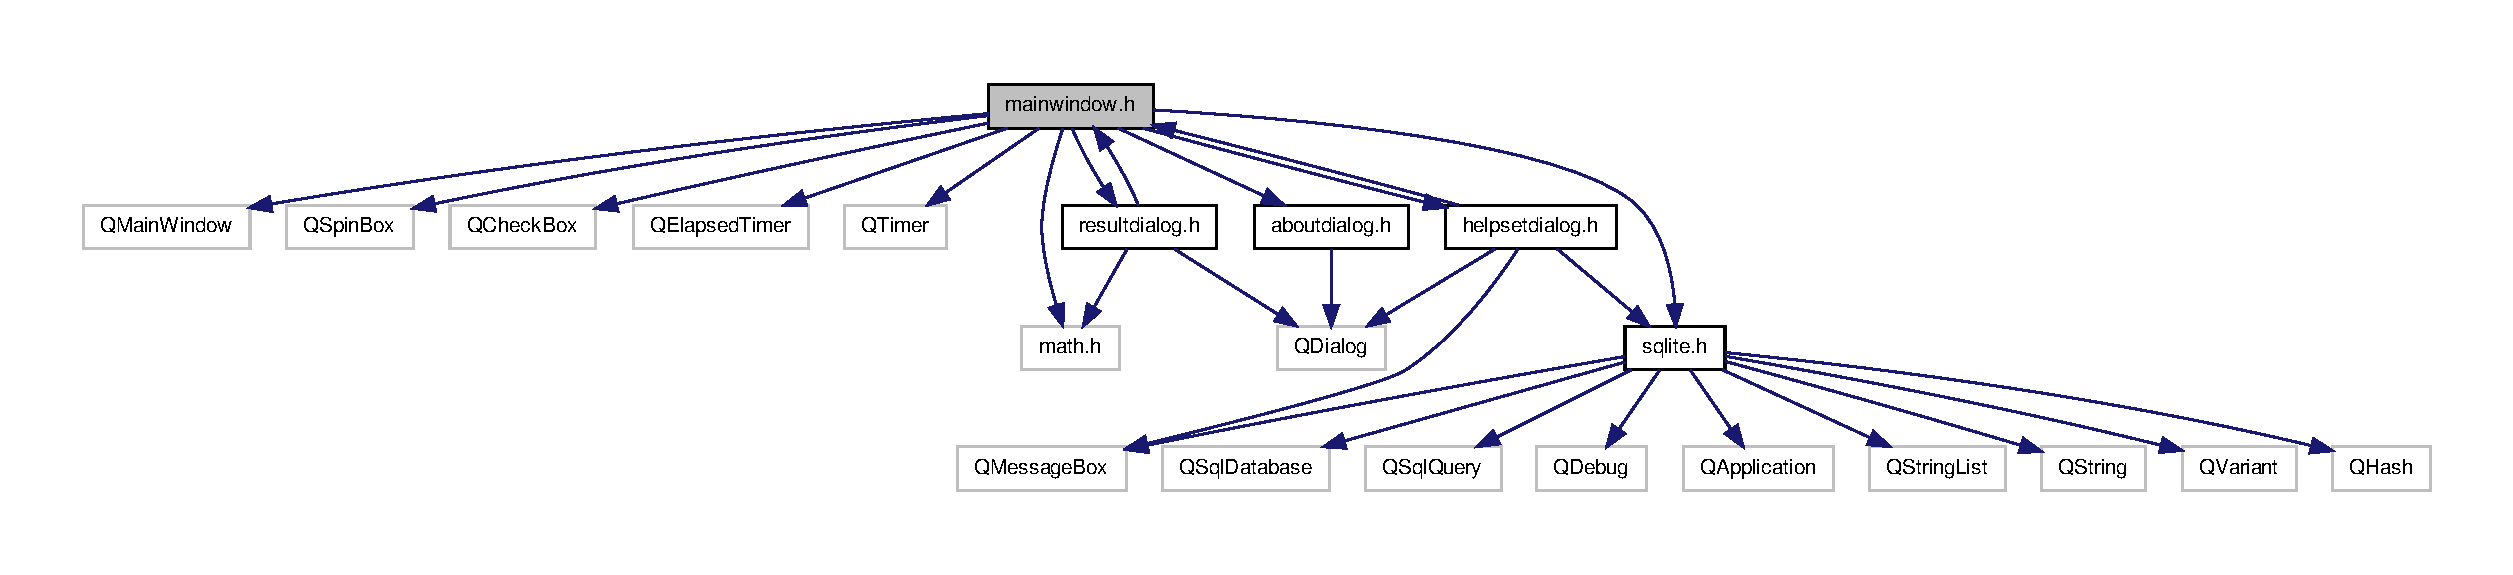
\includegraphics[width=350pt]{mainwindow_8h__incl}
\end{center}
\end{figure}
\-This graph shows which files directly or indirectly include this file\-:\nopagebreak
\begin{figure}[H]
\begin{center}
\leavevmode
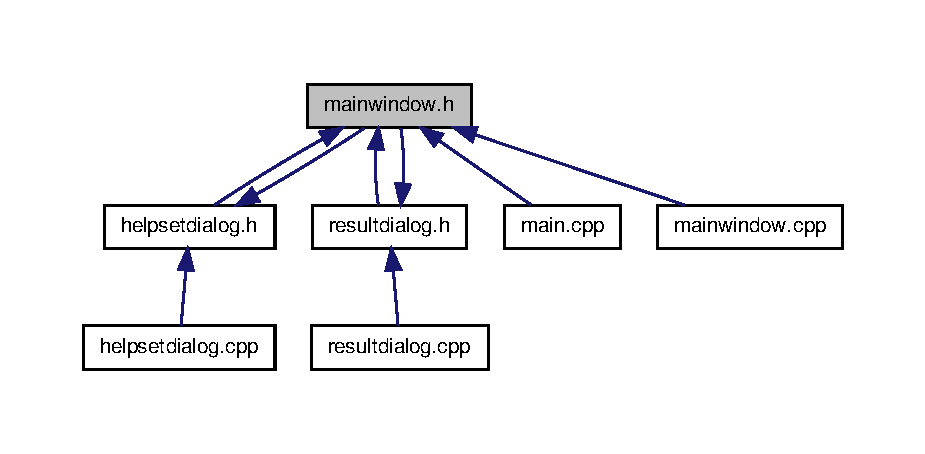
\includegraphics[width=350pt]{mainwindow_8h__dep__incl}
\end{center}
\end{figure}
\subsection*{\-Classes}
\begin{DoxyCompactItemize}
\item 
class \hyperlink{classMainWindow}{\-Main\-Window}
\end{DoxyCompactItemize}
\subsection*{\-Namespaces}
\begin{DoxyCompactItemize}
\item 
namespace \hyperlink{namespacesqlitetest}{sqlitetest}
\item 
namespace \hyperlink{namespaceUi}{\-Ui}
\end{DoxyCompactItemize}
\subsection*{\-Defines}
\begin{DoxyCompactItemize}
\item 
\#define \hyperlink{mainwindow_8h_aa78da16b589b9ca5469c44688b356192}{\-F\-I\-X\-\_\-\-N\-R\-\_\-\-F\-I\-E\-L\-D\-S}~10
\item 
\#define \hyperlink{mainwindow_8h_ad811caf6c72a9a031c67d2af9edc57ab}{\-T\-E\-X\-T\-\_\-\-F\-I\-E\-L\-D\-\_\-\-S\-I\-Z\-E}~1000
\item 
\#define \hyperlink{mainwindow_8h_a475c77257e5782fb60199a7d12a7e53f}{\-M\-A\-X\-\_\-\-R\-E\-C\-O\-R\-D\-S}~5000
\item 
\#define \hyperlink{mainwindow_8h_aff2f9f643149b87035310798f31a5b15}{\-M\-A\-X\-\_\-\-T\-U\-R\-N\-S}~30
\item 
\#define \hyperlink{mainwindow_8h_ab04ce3533c12d8fcbe009e83411d7cee}{\-M\-A\-X\-\_\-\-S\-L\-E\-E\-P\-S}~30
\item 
\#define \hyperlink{mainwindow_8h_afdbfb02687a82624eb0775e9398be734}{\-R\-R\-L\-\_\-\-T\-I\-T\-L\-E}~\char`\"{}\-Ram \-Records \-List \char`\"{}
\item 
\#define \hyperlink{mainwindow_8h_a92c41d772914eb2a3066de8b613bd6c0}{\-D\-R\-L\-\_\-\-T\-I\-T\-L\-E}~\char`\"{}\-Data \-Records \-List \char`\"{}
\end{DoxyCompactItemize}
\subsection*{\-Typedefs}
\begin{DoxyCompactItemize}
\item 
typedef void($\ast$ \hyperlink{mainwindow_8h_a1e88eb4912e990e9280b2045fbf8f190}{\-Anonym\-Void} )()
\end{DoxyCompactItemize}


\subsection{\-Define \-Documentation}
\hypertarget{mainwindow_8h_a92c41d772914eb2a3066de8b613bd6c0}{\index{mainwindow.\-h@{mainwindow.\-h}!\-D\-R\-L\-\_\-\-T\-I\-T\-L\-E@{\-D\-R\-L\-\_\-\-T\-I\-T\-L\-E}}
\index{\-D\-R\-L\-\_\-\-T\-I\-T\-L\-E@{\-D\-R\-L\-\_\-\-T\-I\-T\-L\-E}!mainwindow.h@{mainwindow.\-h}}
\subsubsection[{\-D\-R\-L\-\_\-\-T\-I\-T\-L\-E}]{\setlength{\rightskip}{0pt plus 5cm}\#define {\bf \-D\-R\-L\-\_\-\-T\-I\-T\-L\-E}~\char`\"{}\-Data \-Records \-List \char`\"{}}}\label{mainwindow_8h_a92c41d772914eb2a3066de8b613bd6c0}


\-Definition at line 57 of file mainwindow.\-h.

\hypertarget{mainwindow_8h_aa78da16b589b9ca5469c44688b356192}{\index{mainwindow.\-h@{mainwindow.\-h}!\-F\-I\-X\-\_\-\-N\-R\-\_\-\-F\-I\-E\-L\-D\-S@{\-F\-I\-X\-\_\-\-N\-R\-\_\-\-F\-I\-E\-L\-D\-S}}
\index{\-F\-I\-X\-\_\-\-N\-R\-\_\-\-F\-I\-E\-L\-D\-S@{\-F\-I\-X\-\_\-\-N\-R\-\_\-\-F\-I\-E\-L\-D\-S}!mainwindow.h@{mainwindow.\-h}}
\subsubsection[{\-F\-I\-X\-\_\-\-N\-R\-\_\-\-F\-I\-E\-L\-D\-S}]{\setlength{\rightskip}{0pt plus 5cm}\#define {\bf \-F\-I\-X\-\_\-\-N\-R\-\_\-\-F\-I\-E\-L\-D\-S}~10}}\label{mainwindow_8h_aa78da16b589b9ca5469c44688b356192}


\-Definition at line 51 of file mainwindow.\-h.

\hypertarget{mainwindow_8h_a475c77257e5782fb60199a7d12a7e53f}{\index{mainwindow.\-h@{mainwindow.\-h}!\-M\-A\-X\-\_\-\-R\-E\-C\-O\-R\-D\-S@{\-M\-A\-X\-\_\-\-R\-E\-C\-O\-R\-D\-S}}
\index{\-M\-A\-X\-\_\-\-R\-E\-C\-O\-R\-D\-S@{\-M\-A\-X\-\_\-\-R\-E\-C\-O\-R\-D\-S}!mainwindow.h@{mainwindow.\-h}}
\subsubsection[{\-M\-A\-X\-\_\-\-R\-E\-C\-O\-R\-D\-S}]{\setlength{\rightskip}{0pt plus 5cm}\#define {\bf \-M\-A\-X\-\_\-\-R\-E\-C\-O\-R\-D\-S}~5000}}\label{mainwindow_8h_a475c77257e5782fb60199a7d12a7e53f}


\-Definition at line 53 of file mainwindow.\-h.

\hypertarget{mainwindow_8h_ab04ce3533c12d8fcbe009e83411d7cee}{\index{mainwindow.\-h@{mainwindow.\-h}!\-M\-A\-X\-\_\-\-S\-L\-E\-E\-P\-S@{\-M\-A\-X\-\_\-\-S\-L\-E\-E\-P\-S}}
\index{\-M\-A\-X\-\_\-\-S\-L\-E\-E\-P\-S@{\-M\-A\-X\-\_\-\-S\-L\-E\-E\-P\-S}!mainwindow.h@{mainwindow.\-h}}
\subsubsection[{\-M\-A\-X\-\_\-\-S\-L\-E\-E\-P\-S}]{\setlength{\rightskip}{0pt plus 5cm}\#define {\bf \-M\-A\-X\-\_\-\-S\-L\-E\-E\-P\-S}~30}}\label{mainwindow_8h_ab04ce3533c12d8fcbe009e83411d7cee}


\-Definition at line 55 of file mainwindow.\-h.

\hypertarget{mainwindow_8h_aff2f9f643149b87035310798f31a5b15}{\index{mainwindow.\-h@{mainwindow.\-h}!\-M\-A\-X\-\_\-\-T\-U\-R\-N\-S@{\-M\-A\-X\-\_\-\-T\-U\-R\-N\-S}}
\index{\-M\-A\-X\-\_\-\-T\-U\-R\-N\-S@{\-M\-A\-X\-\_\-\-T\-U\-R\-N\-S}!mainwindow.h@{mainwindow.\-h}}
\subsubsection[{\-M\-A\-X\-\_\-\-T\-U\-R\-N\-S}]{\setlength{\rightskip}{0pt plus 5cm}\#define {\bf \-M\-A\-X\-\_\-\-T\-U\-R\-N\-S}~30}}\label{mainwindow_8h_aff2f9f643149b87035310798f31a5b15}


\-Definition at line 54 of file mainwindow.\-h.

\hypertarget{mainwindow_8h_afdbfb02687a82624eb0775e9398be734}{\index{mainwindow.\-h@{mainwindow.\-h}!\-R\-R\-L\-\_\-\-T\-I\-T\-L\-E@{\-R\-R\-L\-\_\-\-T\-I\-T\-L\-E}}
\index{\-R\-R\-L\-\_\-\-T\-I\-T\-L\-E@{\-R\-R\-L\-\_\-\-T\-I\-T\-L\-E}!mainwindow.h@{mainwindow.\-h}}
\subsubsection[{\-R\-R\-L\-\_\-\-T\-I\-T\-L\-E}]{\setlength{\rightskip}{0pt plus 5cm}\#define {\bf \-R\-R\-L\-\_\-\-T\-I\-T\-L\-E}~\char`\"{}\-Ram \-Records \-List \char`\"{}}}\label{mainwindow_8h_afdbfb02687a82624eb0775e9398be734}


\-Definition at line 56 of file mainwindow.\-h.

\hypertarget{mainwindow_8h_ad811caf6c72a9a031c67d2af9edc57ab}{\index{mainwindow.\-h@{mainwindow.\-h}!\-T\-E\-X\-T\-\_\-\-F\-I\-E\-L\-D\-\_\-\-S\-I\-Z\-E@{\-T\-E\-X\-T\-\_\-\-F\-I\-E\-L\-D\-\_\-\-S\-I\-Z\-E}}
\index{\-T\-E\-X\-T\-\_\-\-F\-I\-E\-L\-D\-\_\-\-S\-I\-Z\-E@{\-T\-E\-X\-T\-\_\-\-F\-I\-E\-L\-D\-\_\-\-S\-I\-Z\-E}!mainwindow.h@{mainwindow.\-h}}
\subsubsection[{\-T\-E\-X\-T\-\_\-\-F\-I\-E\-L\-D\-\_\-\-S\-I\-Z\-E}]{\setlength{\rightskip}{0pt plus 5cm}\#define {\bf \-T\-E\-X\-T\-\_\-\-F\-I\-E\-L\-D\-\_\-\-S\-I\-Z\-E}~1000}}\label{mainwindow_8h_ad811caf6c72a9a031c67d2af9edc57ab}


\-Definition at line 52 of file mainwindow.\-h.



\subsection{\-Typedef \-Documentation}
\hypertarget{mainwindow_8h_a1e88eb4912e990e9280b2045fbf8f190}{\index{mainwindow.\-h@{mainwindow.\-h}!\-Anonym\-Void@{\-Anonym\-Void}}
\index{\-Anonym\-Void@{\-Anonym\-Void}!mainwindow.h@{mainwindow.\-h}}
\subsubsection[{\-Anonym\-Void}]{\setlength{\rightskip}{0pt plus 5cm}typedef void($\ast$ {\bf \-Anonym\-Void})()}}\label{mainwindow_8h_a1e88eb4912e990e9280b2045fbf8f190}


\-Definition at line 59 of file mainwindow.\-h.


\hypertarget{resultdialog_8cpp}{\section{resultdialog.\-cpp \-File \-Reference}
\label{resultdialog_8cpp}\index{resultdialog.\-cpp@{resultdialog.\-cpp}}
}
{\ttfamily \#include \char`\"{}resultdialog.\-h\char`\"{}}\*
{\ttfamily \#include \char`\"{}ui\-\_\-resultdialog.\-h\char`\"{}}\*
\-Include dependency graph for resultdialog.\-cpp\-:\nopagebreak
\begin{figure}[H]
\begin{center}
\leavevmode
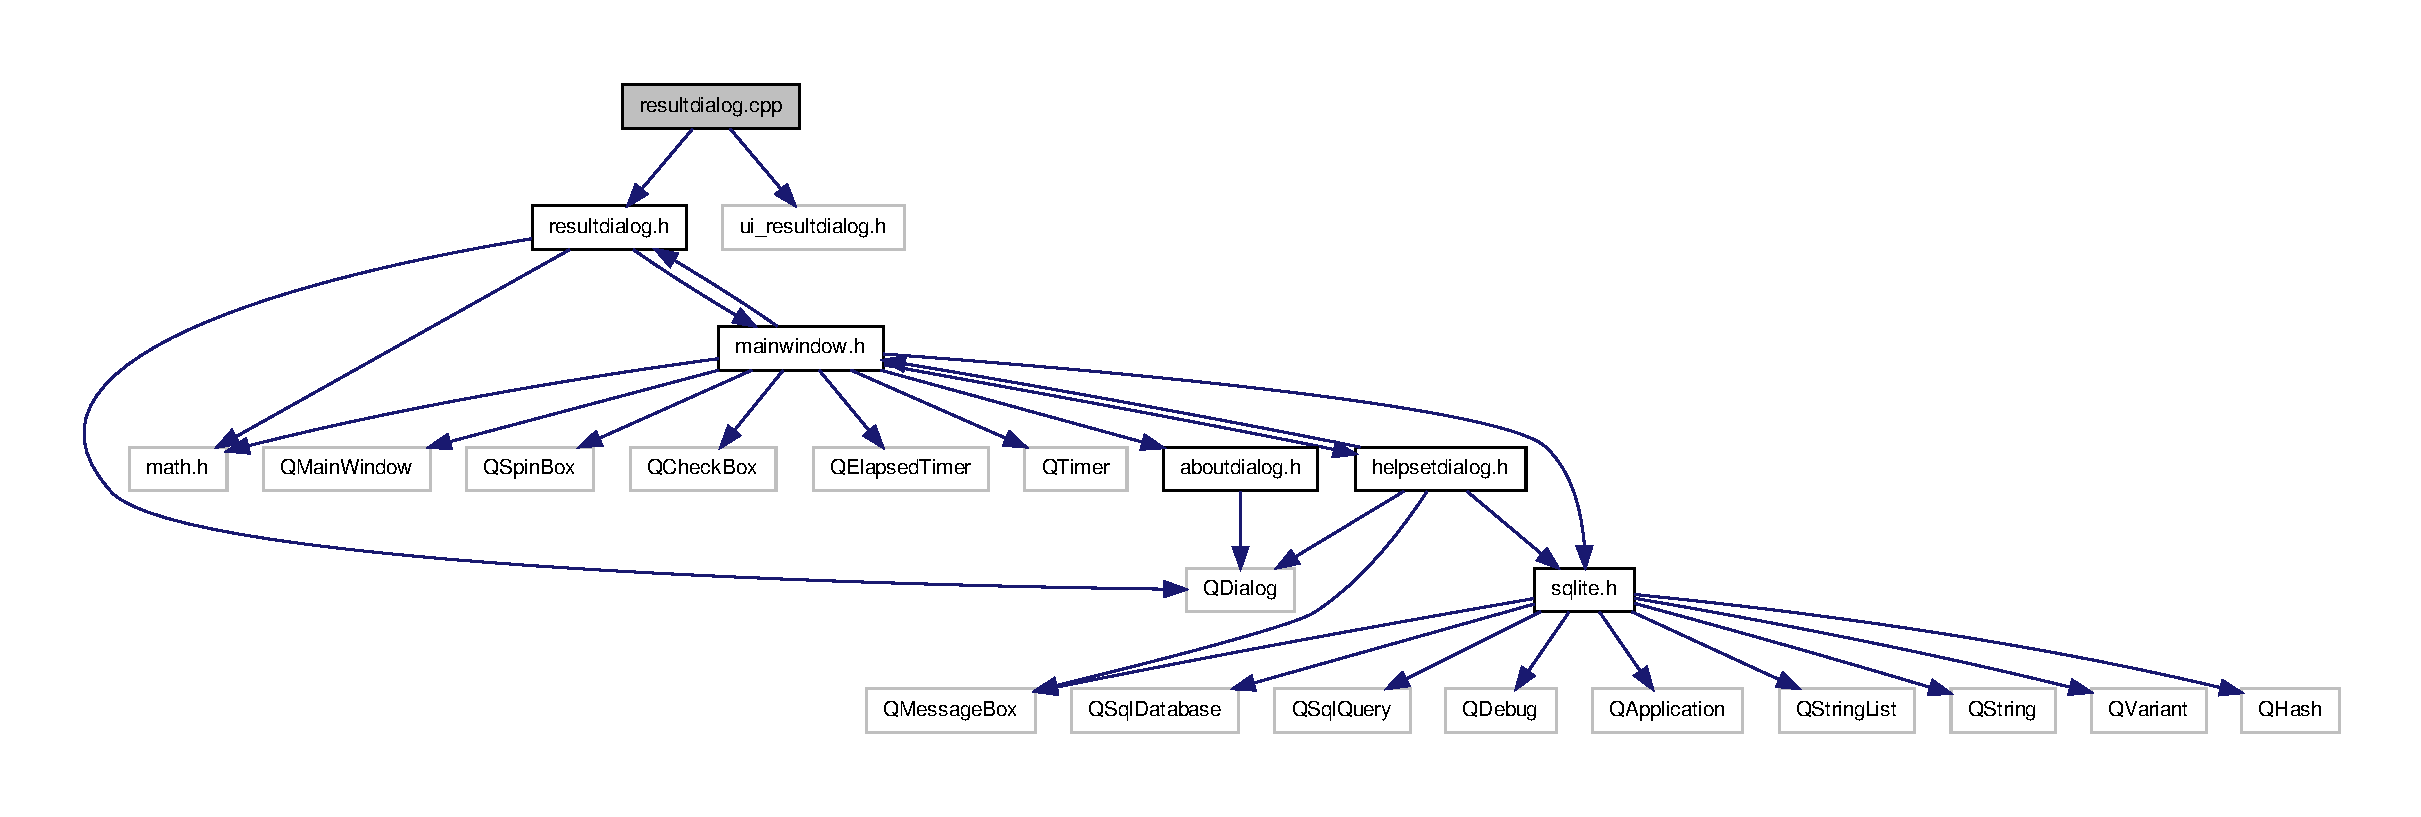
\includegraphics[width=350pt]{resultdialog_8cpp__incl}
\end{center}
\end{figure}
\subsection*{\-Namespaces}
\begin{DoxyCompactItemize}
\item 
namespace \hyperlink{namespacesqlitetest}{sqlitetest}
\end{DoxyCompactItemize}

\hypertarget{resultdialog_8h}{\section{resultdialog.\-h \-File \-Reference}
\label{resultdialog_8h}\index{resultdialog.\-h@{resultdialog.\-h}}
}
{\ttfamily \#include $<$\-Q\-Dialog$>$}\*
{\ttfamily \#include $<$math.\-h$>$}\*
{\ttfamily \#include \char`\"{}mainwindow.\-h\char`\"{}}\*
\-Include dependency graph for resultdialog.\-h\-:\nopagebreak
\begin{figure}[H]
\begin{center}
\leavevmode
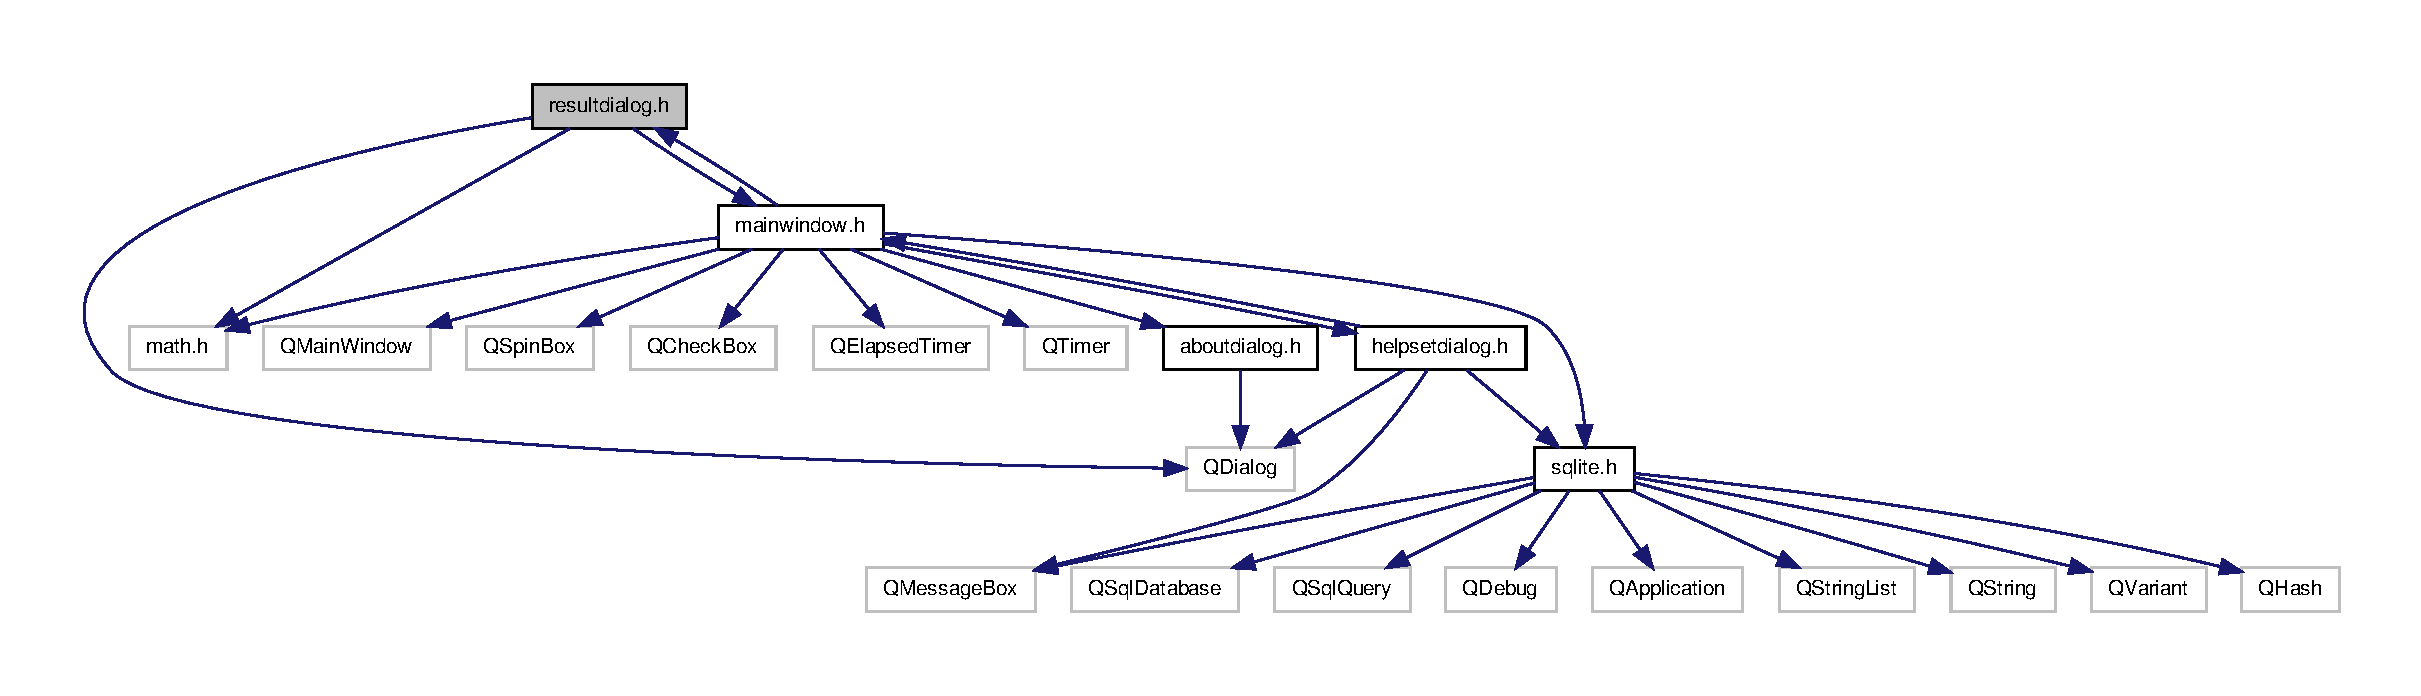
\includegraphics[width=350pt]{resultdialog_8h__incl}
\end{center}
\end{figure}
\-This graph shows which files directly or indirectly include this file\-:\nopagebreak
\begin{figure}[H]
\begin{center}
\leavevmode
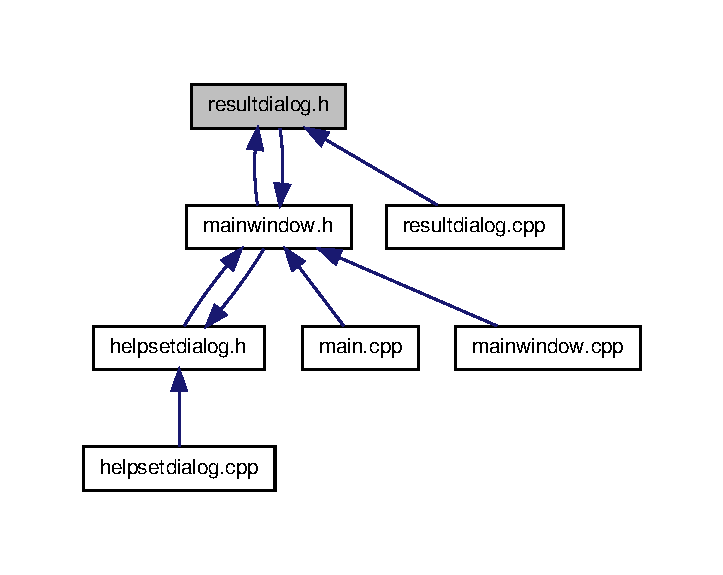
\includegraphics[width=347pt]{resultdialog_8h__dep__incl}
\end{center}
\end{figure}
\subsection*{\-Classes}
\begin{DoxyCompactItemize}
\item 
class \hyperlink{classResultDialog}{\-Result\-Dialog}
\end{DoxyCompactItemize}
\subsection*{\-Namespaces}
\begin{DoxyCompactItemize}
\item 
namespace \hyperlink{namespacesqlitetest}{sqlitetest}
\item 
namespace \hyperlink{namespaceUi}{\-Ui}
\end{DoxyCompactItemize}

\hypertarget{sqlite_8cpp}{\section{sqlite.\-cpp \-File \-Reference}
\label{sqlite_8cpp}\index{sqlite.\-cpp@{sqlite.\-cpp}}
}
{\ttfamily \#include \char`\"{}sqlite.\-h\char`\"{}}\*
{\ttfamily \#include $<$\-Q\-Dir$>$}\*
{\ttfamily \#include $<$\-Q\-Elapsed\-Timer$>$}\*
\-Include dependency graph for sqlite.\-cpp\-:\nopagebreak
\begin{figure}[H]
\begin{center}
\leavevmode
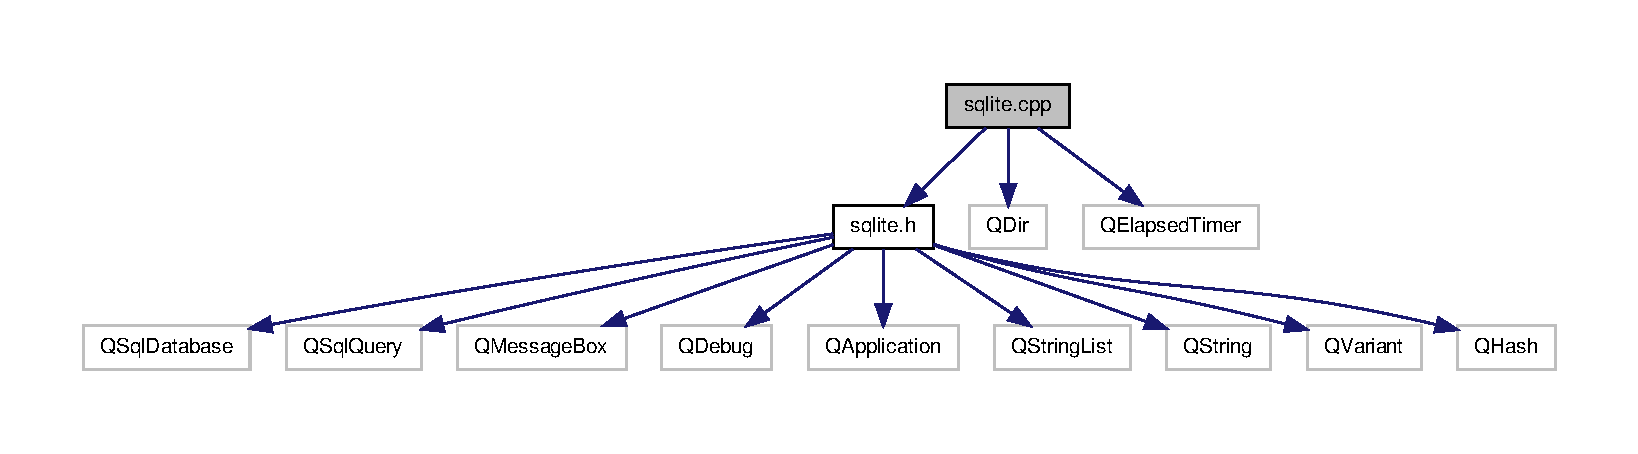
\includegraphics[width=350pt]{sqlite_8cpp__incl}
\end{center}
\end{figure}
\subsection*{\-Namespaces}
\begin{DoxyCompactItemize}
\item 
namespace \hyperlink{namespacesqlitetest}{sqlitetest}
\end{DoxyCompactItemize}

\hypertarget{sqlite_8h}{\section{sqlite.\-h \-File \-Reference}
\label{sqlite_8h}\index{sqlite.\-h@{sqlite.\-h}}
}
{\ttfamily \#include $<$\-Q\-Sql\-Database$>$}\*
{\ttfamily \#include $<$\-Q\-Sql\-Query$>$}\*
{\ttfamily \#include $<$\-Q\-Message\-Box$>$}\*
{\ttfamily \#include $<$\-Q\-Debug$>$}\*
{\ttfamily \#include $<$\-Q\-Application$>$}\*
{\ttfamily \#include $<$\-Q\-String\-List$>$}\*
{\ttfamily \#include $<$\-Q\-String$>$}\*
{\ttfamily \#include $<$\-Q\-Variant$>$}\*
{\ttfamily \#include $<$\-Q\-Hash$>$}\*
\-Include dependency graph for sqlite.\-h\-:\nopagebreak
\begin{figure}[H]
\begin{center}
\leavevmode
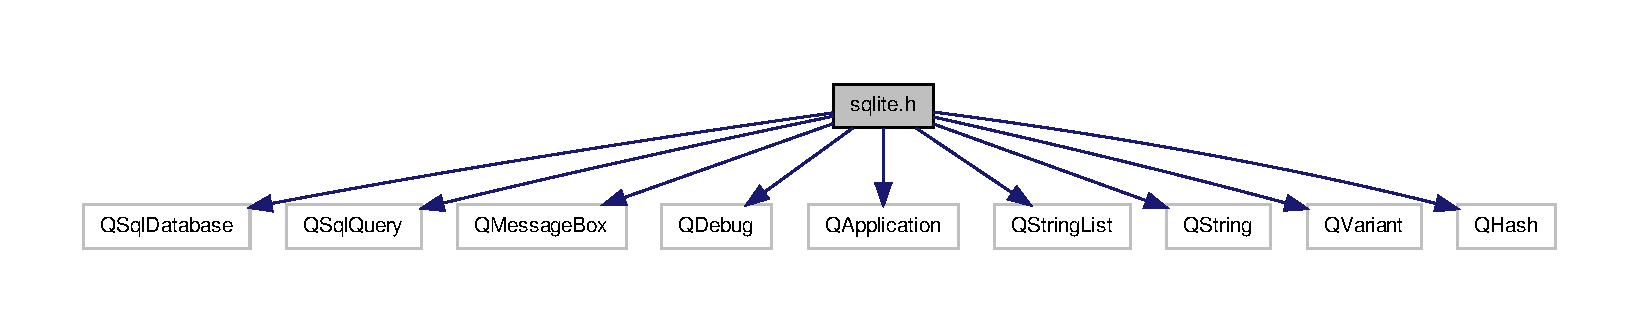
\includegraphics[width=350pt]{sqlite_8h__incl}
\end{center}
\end{figure}
\-This graph shows which files directly or indirectly include this file\-:\nopagebreak
\begin{figure}[H]
\begin{center}
\leavevmode
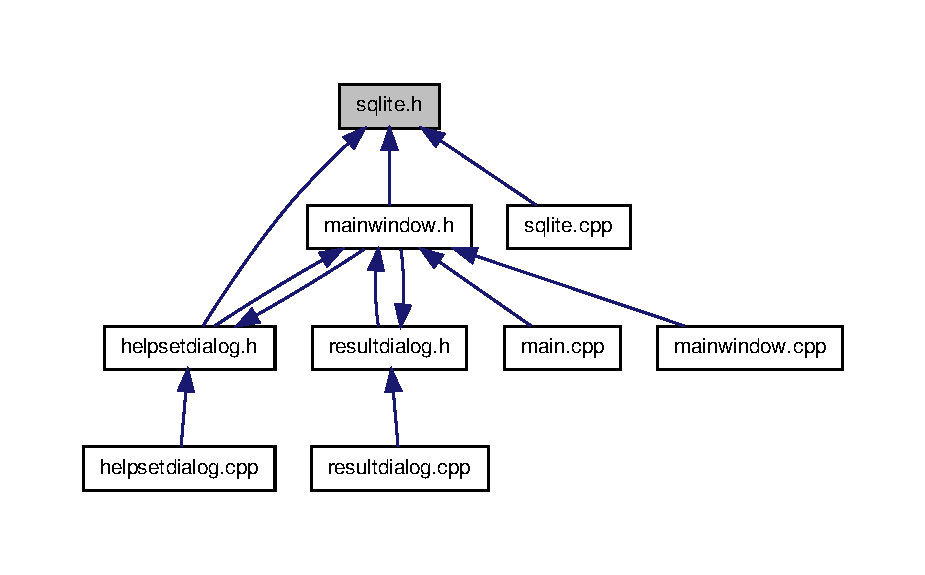
\includegraphics[width=350pt]{sqlite_8h__dep__incl}
\end{center}
\end{figure}
\subsection*{\-Classes}
\begin{DoxyCompactItemize}
\item 
struct \hyperlink{structSqlPreferences}{\-Sql\-Preferences}
\item 
class \hyperlink{classSQLite}{\-S\-Q\-Lite}
\end{DoxyCompactItemize}
\subsection*{\-Namespaces}
\begin{DoxyCompactItemize}
\item 
namespace \hyperlink{namespacesqlitetest}{sqlitetest}
\end{DoxyCompactItemize}
\subsection*{\-Defines}
\begin{DoxyCompactItemize}
\item 
\#define \hyperlink{sqlite_8h_acfcad24977a121f8cb40c7abc0861e13}{\-D\-E\-F\-A\-U\-L\-T\-\_\-\-D\-B\-N\-A\-M\-E}~\char`\"{}/testdb.\-db3\char`\"{}
\item 
\#define \hyperlink{sqlite_8h_adda28390da72cdfef24377fcd0262e17}{\-D\-E\-F\-A\-U\-L\-T\-\_\-\-T\-A\-B\-L\-E\-N\-A\-M\-E}~\char`\"{}testdb\char`\"{}
\end{DoxyCompactItemize}


\subsection{\-Define \-Documentation}
\hypertarget{sqlite_8h_acfcad24977a121f8cb40c7abc0861e13}{\index{sqlite.\-h@{sqlite.\-h}!\-D\-E\-F\-A\-U\-L\-T\-\_\-\-D\-B\-N\-A\-M\-E@{\-D\-E\-F\-A\-U\-L\-T\-\_\-\-D\-B\-N\-A\-M\-E}}
\index{\-D\-E\-F\-A\-U\-L\-T\-\_\-\-D\-B\-N\-A\-M\-E@{\-D\-E\-F\-A\-U\-L\-T\-\_\-\-D\-B\-N\-A\-M\-E}!sqlite.h@{sqlite.\-h}}
\subsubsection[{\-D\-E\-F\-A\-U\-L\-T\-\_\-\-D\-B\-N\-A\-M\-E}]{\setlength{\rightskip}{0pt plus 5cm}\#define {\bf \-D\-E\-F\-A\-U\-L\-T\-\_\-\-D\-B\-N\-A\-M\-E}~\char`\"{}/testdb.\-db3\char`\"{}}}\label{sqlite_8h_acfcad24977a121f8cb40c7abc0861e13}


\-Definition at line 51 of file sqlite.\-h.

\hypertarget{sqlite_8h_adda28390da72cdfef24377fcd0262e17}{\index{sqlite.\-h@{sqlite.\-h}!\-D\-E\-F\-A\-U\-L\-T\-\_\-\-T\-A\-B\-L\-E\-N\-A\-M\-E@{\-D\-E\-F\-A\-U\-L\-T\-\_\-\-T\-A\-B\-L\-E\-N\-A\-M\-E}}
\index{\-D\-E\-F\-A\-U\-L\-T\-\_\-\-T\-A\-B\-L\-E\-N\-A\-M\-E@{\-D\-E\-F\-A\-U\-L\-T\-\_\-\-T\-A\-B\-L\-E\-N\-A\-M\-E}!sqlite.h@{sqlite.\-h}}
\subsubsection[{\-D\-E\-F\-A\-U\-L\-T\-\_\-\-T\-A\-B\-L\-E\-N\-A\-M\-E}]{\setlength{\rightskip}{0pt plus 5cm}\#define {\bf \-D\-E\-F\-A\-U\-L\-T\-\_\-\-T\-A\-B\-L\-E\-N\-A\-M\-E}~\char`\"{}testdb\char`\"{}}}\label{sqlite_8h_adda28390da72cdfef24377fcd0262e17}


\-Definition at line 52 of file sqlite.\-h.


\printindex
\end{document}
